\chapter{急性腹痛}

急性腹痛是常见的临床症状。引起急性腹痛的原因,可分为两类:①由于腹内脏器病变所致者;②由于腹外脏器或全身性病变所致者。由于腹内脏器病变所致者,又可再分为器质性与功能性两组。前者包括脏器的炎症、穿孔、破裂、梗阻、套叠、扭转、绞窄等,其中有外科情况者临床上称之为“急腹症”。引起急性腹痛的疾病很多,其共同特点是发病急、变化快和病情重。本章所讨论的以内科临床医生需要了解的知识为范围。

急性腹痛疾病的诊断流程一般可分为两个步骤:

1.迅速作细致的病史询问、体格检查和有选择地作一些必要的辅助检查。

2.综合全面材料进行分析,确定病变的部位、性质和病因,作为治疗的依据。

急性腹痛的病因及其临床表现虽错综复杂,但下列的一些特点和规律,可有助于鉴别诊断:

\section{【问诊】}

\subsection{(一)急性腹痛与发病年龄、性别、婚否、职业的关系}

如肠套叠、嵌顿性腹股沟疝、蛔虫性肠梗阻、胆道蛔虫病等以幼年期多见,尤其多见于农村儿童;急性阑尾炎、急性胰腺炎、胃十二指肠溃疡急性穿孔以青壮年多见;胆囊炎、胆石症、消化系统恶性肿瘤以中、老年人多见。卵巢囊肿扭转、急性输卵管炎是女性疾病。异位妊娠破裂发生于有性生活史的生育期女性。重金属(铅、砷等)中毒性腹痛有长期的或过量重金属接触史。

\subsection{(二)既往病史和起病诱因}

胃十二指肠溃疡穿孔常有慢性上腹痛史,胆绞痛、肾绞痛等常可追溯以往有类似发作的病史。胆道蛔虫病与蛔虫性肠梗阻患者常有排蛔虫或吐蛔虫史。急性肠套叠常与突然改变饮食有关。胃十二指肠溃疡穿孔、急性胰腺炎、急性胃扩张,常因暴饮暴食而激发。胆绞痛往往见于进食肥腻食物(尤其是用油煎炸的)后发作。急性缺血性肠病常见于高血压、糖尿病患者。既往有腹部手术史或结核性腹膜炎史者须考虑机械性肠梗阻的诊断。功能性胃肠疾病患者常有饮食不节、精神紧张、情绪不稳、工作压力大、失眠等诱因。

\subsection{(三)急性腹痛的部位}

有些急性腹痛的患者就诊时常能明确指出腹痛的部位。最先出现腹痛的部位大多数是病变的所在,如胃十二指肠溃疡穿孔、胆囊炎、胆石症、胆道蛔虫病等。为了临床鉴别诊断的需要,将急性腹痛部位与疾病的关系分八个腹部分区(图\ref{fig25-1},表\ref{tab25-1}),以供参考。在临床上,发现腹痛部位与疾病的关系不明显者不少,如急性阑尾炎开始时疼痛在中上腹部或脐周围,以后才转移到右下腹(但值得注意的是,其他疾病引起的腹痛也可表现为转移性腹痛);网膜、回肠下段等器官同受第十胸神经节支配,这些器官发生炎症等病变时,疼痛最初部位不确定或在中上腹部或脐周,以后才局限于发炎器官的所在部位。固定性压痛对确定病变部位更有重要意义,如阑尾绞痛位于阑尾压痛点(麦氏点),即使阑尾炎发病初期,腹痛表现为上腹痛,但固定压痛点仍以右下腹麦氏点最为明显。胆绞痛位于右上腹胆囊区,向右侧背部放射;肾绞痛位于肾区,沿输尿管向外阴部放射;小肠绞痛常位于脐周;大肠绞痛常位于下腹部(图\ref{fig25-2})。还应注意的是有些疾病虽然表现为急性腹痛,而病变却在腹外器官,如大叶性肺炎、胸膜炎、气胸、急性心肌梗死、急性心包炎等。

\begin{figure}[!htbp]
 \centering
 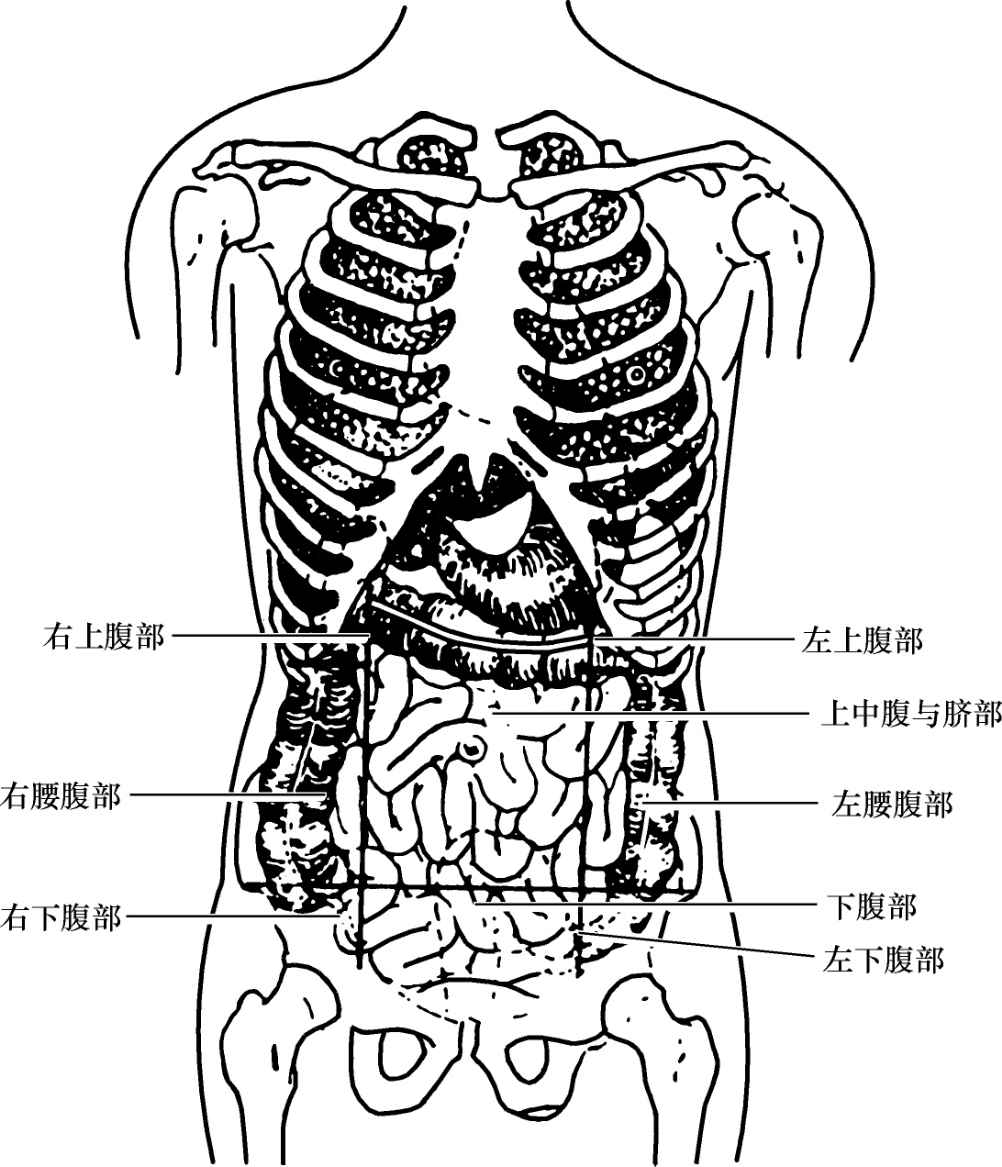
\includegraphics[width=3.27083in,height=3.8125in]{./images/Image00136.jpg}
 \captionsetup{justification=centering}
 \caption{腹部分区示意图}
 \label{fig25-1}
  \end{figure} 

\begin{figure}[!htbp]
 \centering
 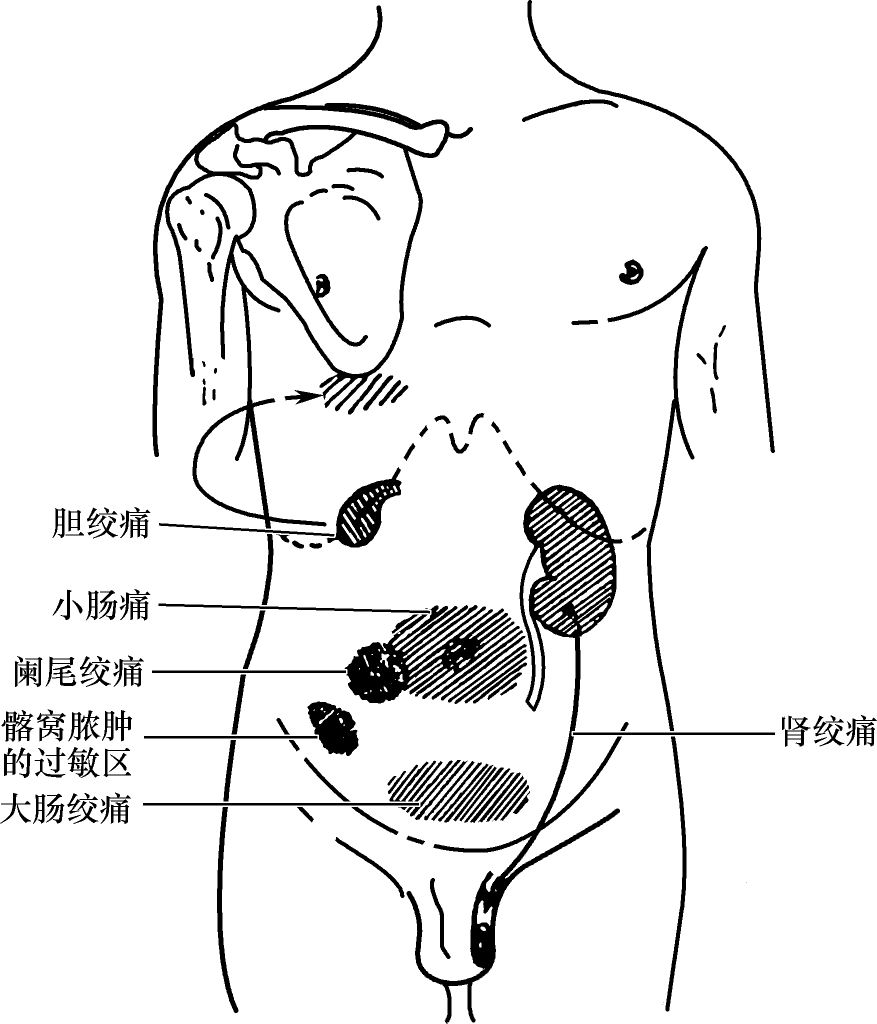
\includegraphics[width=2.625in,height=3.0625in]{./images/Image00137.jpg}
 \captionsetup{justification=centering}
 \caption{各种绞痛的常见部位}
 \label{fig25-2}
  \end{figure} 

\subsection{(四)急性腹痛的时间、性质与程度等}

胃十二指肠溃疡穿孔多在冬、春季节病情恶化之际,突然发生剧烈的刀割样、烧灼样、持续性中上腹疼痛,常被迫静卧以减轻疼痛。夜间中上腹疼痛,尤其向腰背部放射者,要注意胰腺疾病可能;胆绞痛、肾绞痛与肠绞痛是逐渐加剧,迅速达到高峰,疼痛极其剧烈,患者常辗转不安、呻吟、冷汗淋漓,持续若干时间后而逐渐缓解;疼痛常为间歇性,肠绞痛往往持续数分钟,肾绞痛与胆绞痛持续1/2~1小时或以上方能缓解。阵发性钻顶样疼痛是胆道、胰管或阑尾蛔虫梗阻的特征。持续性急性腹痛多是腹腔内炎症性疾病,如急性阑尾炎、急性胰腺炎、急性腹膜炎等。结肠与小肠急性炎症时也常发生绞痛,但往往伴有腹泻。在持续性疼痛的基础上阵发性加剧,多表示伴有梗阻,如胆道结石合并感染。

\begin{table}[htbp]
\centering
\caption{急性腹痛部位与疾病的关系}
\label{tab25-1}
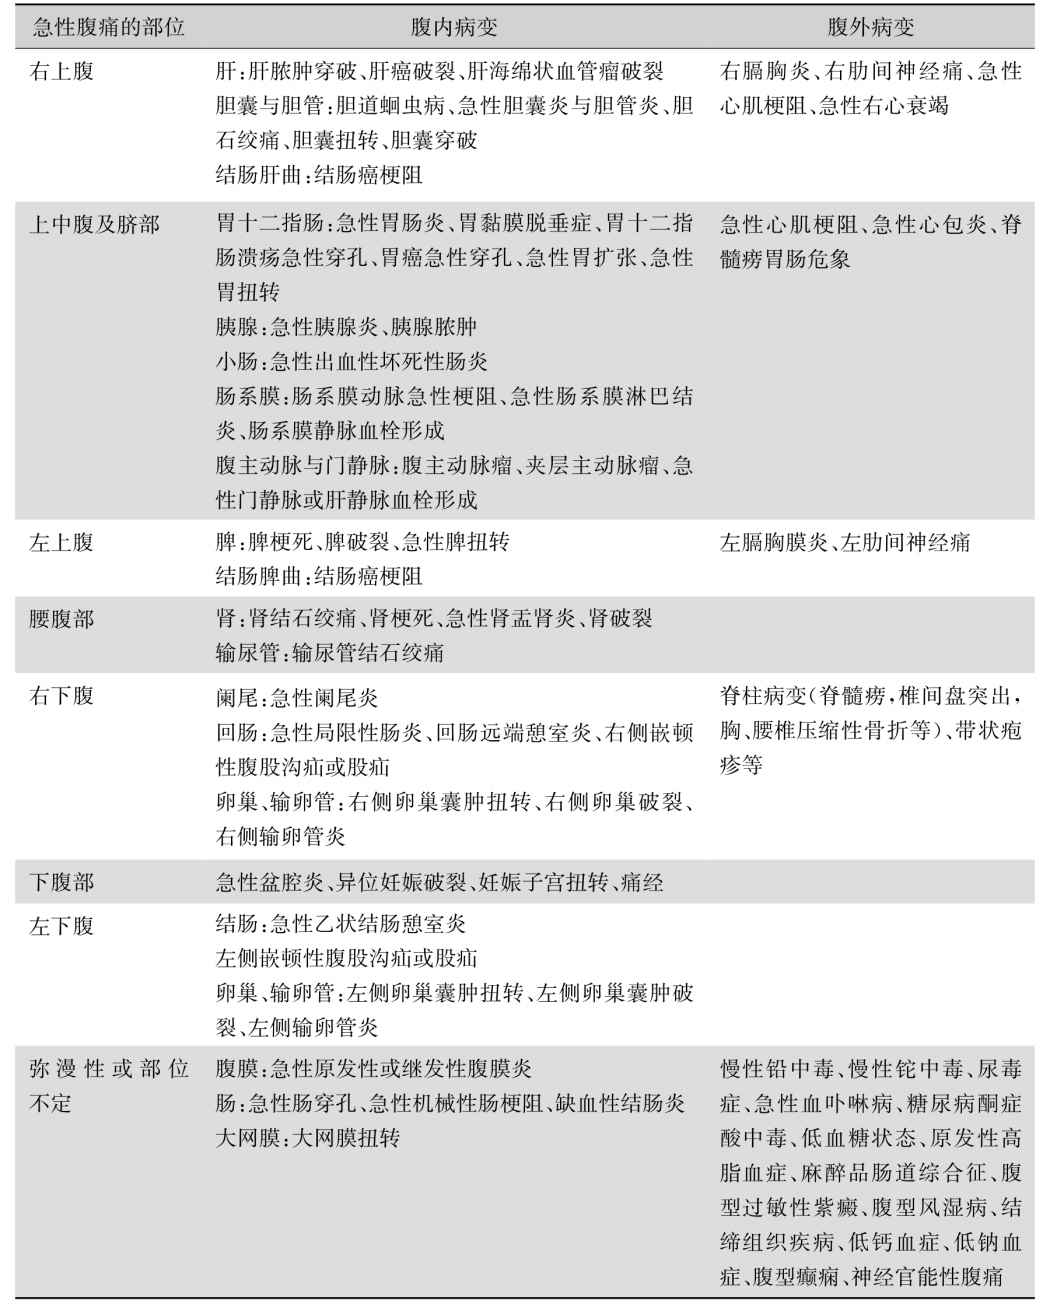
\includegraphics[width=5.94792in,height=7.48958in]{./images/Image00138.jpg}
\end{table}

\subsection{(五)急性腹痛的放射痛}

某些急腹症有特定部位的放射痛,对诊断有一定的参考价值。约半数胆囊炎、胆石症的疼痛向右肩背部放射;胰腺炎的疼痛往往向左腰背部放射;约1/3胃十二指肠溃疡急性穿孔因膈肌腹面受刺激而感肩痛。子宫与直肠痛常放射至腰骶部(图\ref{fig25-3})。输尿管结石绞痛常向会阴部或大腿内侧放射。肩顶痛可能为肝脓肿向横膈穿破前的唯一病征。

\begin{figure}[!htbp]
 \centering
 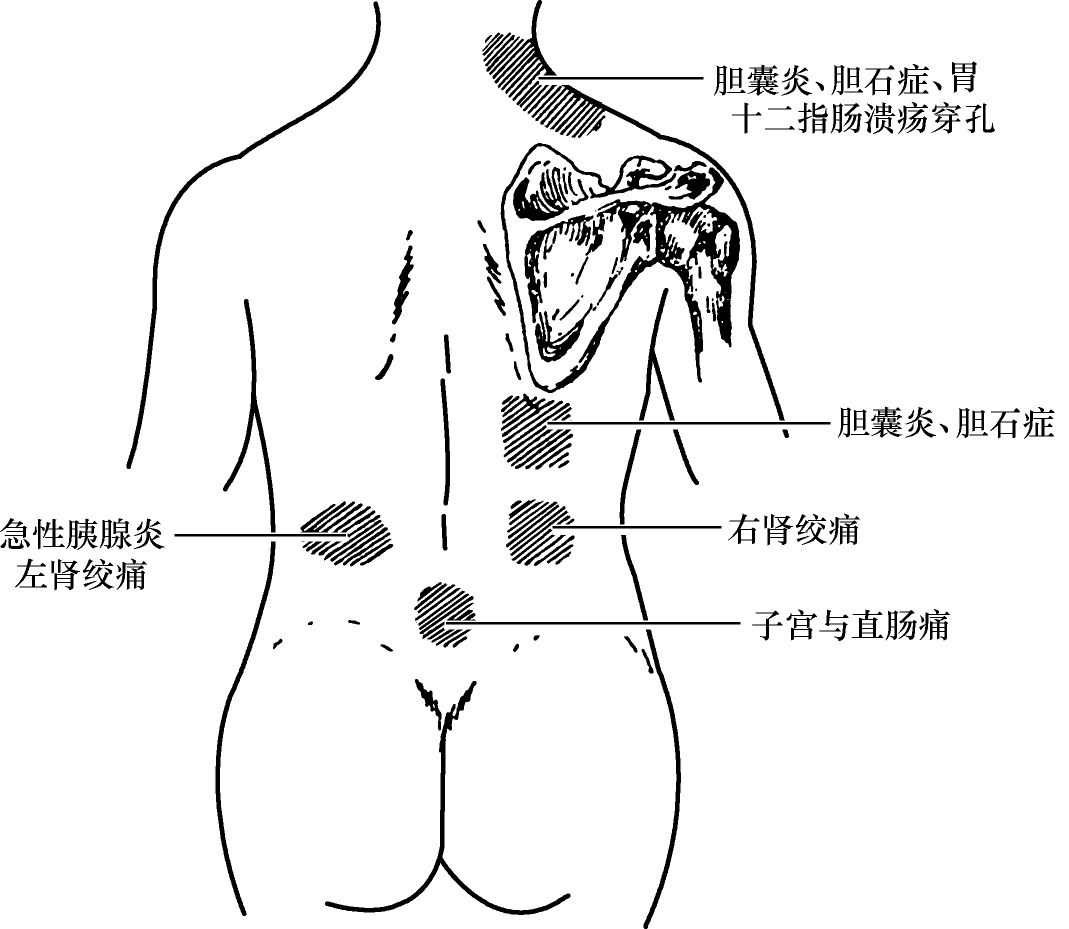
\includegraphics[width=3.55208in,height=3.09375in]{./images/Image00139.jpg}
 \captionsetup{justification=centering}
 \caption{与急性腹部疾病有关的背部疼痛区}
 \label{fig25-3}
  \end{figure} 

\subsection{(六)急性腹痛与伴随症状的关系}

急性腹痛伴血尿,常是泌尿系疾病,如肾或输尿管结石所致的肾绞痛。急性腹痛伴腹泻,除常见的急性胃肠炎(包括细菌性食物中毒)与急性中毒之外,须注意急性阑尾炎、急性盆腔炎。急性腹痛伴呕吐、腹胀、肛门停止排气排便,提示为肠梗阻。急性腹痛伴血便,应注意肠套叠、绞窄性肠梗阻、急性出血坏死性肠炎、缺血性“结肠炎”、腹腔内大血管急性阻塞。急性腹痛伴有发热、畏寒,多表示出现炎症、感染或肿瘤,如胆道结石合并感染;伴有寒战、高热,应考虑感染,如急性梗阻性化脓性胆管炎、腹腔脏器脓肿、大叶性肺炎等疾病。急腹症开始即有高热者,不大支持胃肠穿孔之急性腹膜炎的诊断。急性腹痛伴休克,需注意急性内出血、急性梗阻性化脓性胆管炎、急性胰腺炎、绞窄性肠梗阻、胃十二指肠溃疡急性出血、腹腔脏器扭转或急性心肌梗死等情况(图\ref{fig25-4})。神经性或中枢神经系统疾病所致的腹痛,可伴有腹腔外症状,如腹型癫痫,部分患者有癫痫的其他症状;皮肤对称性、成批出现出血性皮疹,尤其是双下肢,提示过敏性紫癜;功能性腹痛常有敏感、多疑和精神紧张的特征。

\begin{figure}[!htbp]
 \centering
 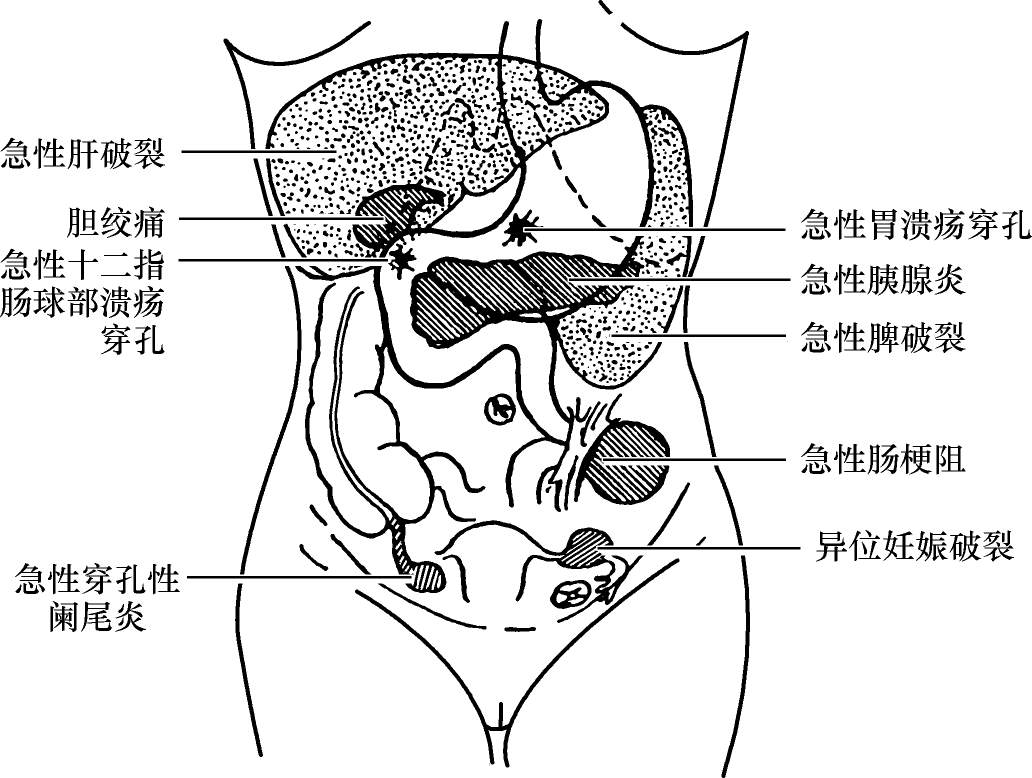
\includegraphics[width=3.4375in,height=2.58333in]{./images/Image00140.jpg}
 \captionsetup{justification=centering}
 \caption{较常引起休克的急性腹痛}
 \label{fig25-4}
  \end{figure} 

\section{【体格检查】}

\subsection{(一)一般检查}

面部表情常能提示疼痛的程度。希(Hippocrates)氏面容(表情痛苦、面色灰白、两眼无神、额部冷汗、眼球凹陷、两颧突出、鼻尖峭立)常为急性弥漫性腹膜炎的病征。但须注意,胃十二指肠溃疡穿孔如出现休克或急性弥漫性腹膜炎,患者可能感觉腹痛反而明显减轻。梗阻性疾病绞痛发作时,患者辗转不安,呻吟不已。急性腹膜炎患者常为减轻疼痛而蜷曲侧卧,不敢随意转身或活动。生育期已婚妇女出现下腹痛伴面色苍白、呼吸加速、脉搏细数等外周循环功能不足症状,而无发热者,应注意异位妊娠破裂或黄体破裂出血的可能。右上腹痛伴黄疸,有助于肝、胆道及胰腺疾病的诊断;中上腹痛伴黄疸,有利于胰腺疾病的诊断;右上腹痛伴黄疸、发热、寒战,须注意右下叶肺炎、膈下脓肿、肝脓肿、急性肝胆道炎症等。脉搏细数常见于腹腔脏器急性炎症性或出血性疾病(可能与交感神经兴奋有关)。脉慢而弦常见于腹腔脏器的绞痛(可能与副交感神经兴奋有关)。外科急腹症,开始体温多为正常,以后因并发感染而体温升高,但如合并休克,也可无发热,甚至反而出现体温不升。皮肤皮疹或出血点,对病因的诊断非常重要,如过敏性紫癜(腹型)等。

\subsection{(二)胸部检查}

心肺的体格检查(包括视、触、叩、听诊)在急腹症时不应忽略。

\subsection{(三)腹部检查}

视诊时宜裸露全腹(天气寒冷时应注意保暖),以免遗漏嵌顿性腹股沟疝或股疝。急性腹膜炎时,腹式呼吸运动减弱或完全消失。舟状腹见于急性胃肠溃疡穿孔的早期或合并慢性消耗性疾病。全腹膨隆是肠梗阻、肠麻痹、晚期腹膜炎的体征;中上腹部胀满,可见于急性胃扩张或胃潴留;局部不对称的腹胀可见于闭袢性肠梗阻、肠扭转、缺血性结肠炎、腹腔或盆腔肿瘤等。胆囊肿大时,可见到随呼吸运动而上下移动的右上腹梨形包块。正常胃蠕动波从左肋缘开始,缓慢向右下方移动,最后消失于幽门区;幽门梗阻时,上腹部可见胃型及可能出现的反方向胃蠕动波。肠型、肠蠕动波是肠梗阻的征象。小肠梗阻时,可见到阶梯式蠕动波,伴同肠绞痛而出现。

触诊发现肌紧张、压痛与反跳痛,是炎症波及腹膜壁层的常见体征。急性胃、肠穿孔,腹壁常呈板样硬(板状腹);胰腺是腹腔深部器官,急性胰腺炎时,腹肌紧张一般为轻度至中度。腹肌紧张以细菌性腹膜炎和化学性腹膜炎最明显,其次为阿米巴性腹膜炎,而腹腔内出血时较轻。但须注意,当腹壁脂肪厚而松弛、或肌肉不发达、或有重度毒血症或全身衰竭患者(尤其是老年患者),虽有重症腹膜炎而腹肌紧张等腹肌刺激征可能较轻。腹部压痛最明显处往往是病变所在,触诊发现局部压痛,宜与健侧或其他部位作比较,宜排除患者因感觉过敏而出现误判。急性阑尾炎早期炎症病征不明显时,触诊应与健侧对比,往往能获得较深刻的印象。急性腹膜炎患者常拒按,而铅毒性绞痛患者往往喜按。触诊发现肿块,首先应排除正常脏器,如剑突、肠道积粪、腹主动脉、脊柱、下垂肾脏等,病理情况可见于炎症性包块、肿大的胆囊或粘连的肠袢、肠套叠、囊肿的扭转或肿瘤。值得重视的是,直肠指检对诊断盆腔内炎性肿块、脓肿、肿瘤以及肠套叠等往往有重要的帮助。

叩诊发现肝浊音界缩小或消失,是急性胃、肠穿孔或高度肠胀气的体征。移动性浊音提示有腹腔液体存在,应考虑:①腹水(渗出液或漏出液),常见于肝硬化腹水、各种原因腹膜炎性渗出液或巨大脓肿向腹腔穿破;②内出血,如肿瘤破裂出血、异位妊娠破裂出血等。腹腔穿刺适用于诊断原因未明的腹腔积液,例如疑有腹腔内出血或腹膜炎症性渗出液时。叩诊鼓音提示腹腔气体增多,如各种原因气腹(包括人工气腹或某些微创手术后)、肠梗阻等。

听诊时如听到肠鸣音活跃,是肠蠕动增强的表现,可能是生理性的,如禁食、服用胃肠动力药物等;也可能是病理性的,如急性肠炎、消化道出血等;如出现高亢、气过水声、金属音等常见于机械性肠梗阻。反之,肠鸣音高度减弱或消失,是肠麻痹的体征,常见于急性(重症)腹膜炎或各种原因所致麻痹性肠梗阻;如患者肠鸣音由高亢、气过水声、金属音变为肠鸣音减弱、消失,尤其是患者一般情况恶化时,应注意很可能出现绞窄性肠梗阻、肠坏死。值得重视的是,近年来,一些药物,包括各种解痉药(如抗胆碱药等)和生长抑素使用后,可导致肠鸣音减弱,影响临床对病情及预后的判断与评估(如消化道出血或肿瘤所致机械性肠梗阻应用生长抑素后影响病情观察)。

\section{【实验室检查】}

尿常规与血常规是例行的检查。尿比重增高常提示失水,是补液的指征。蛋白尿、糖尿、尿酮体、脓尿、血尿、血红蛋白尿以及卟啉尿等的出现,均为诊断的重要线索。尿与血清淀粉酶、脂肪酶增高对诊断急性胰腺炎有决定性意义。血便或黑便对于消化道溃疡、肠道炎症(包括感染性肠病、炎症性肠病、出血坏死性小肠炎、缺血性肠病等)、肿瘤等诊断非常有帮助;怀疑胆道蛔虫病、蛔虫性肠梗阻、肝阿米巴病时,须即作粪便镜检。白细胞血象可提供急性腹痛由于感染性或非感染性疾病,炎症性或非炎症性疾病的根据;中重度贫血,尤其是正细胞、正色素贫血,提示内出血或血液病可能。妊娠试验阳性的腹痛患者,尤其是合并有腹膜刺激征或(和)腹腔内出血的患者,高度提示异位妊娠破裂出血的诊断。肝功能,肝酶学和胆红素升高,尤其是胆红素、ALP、GGT等升高,提示肝胆胰疾病。心肌酶升高提示急性心肌梗死。

\section{【影像学检查】}

B超、X线胸、腹部透视、腹部平片检查、CT、MRI、心电图以及近年来广泛应用于临床的超声内镜等检查应作为例行筛选检查,常能提供重要的诊断根据。B超检查有助于提示腹腔内积液、肿块、结石的诊断;各型超声扫描有助于鉴别异位妊娠破裂出血与其他原因的内出血。X线腹平片对于肠梗阻、胃肠穿孔和某些结石病有诊断价值;CT、MRI能提示不仅能发现腹腔实质脏器病变,而且可提示大血管病变。心电图描记有助于急性心肌梗死的诊断。超声内镜有助于发现和明确胰胆管和腹腔病灶的检出和诊断。

\section{【分析、诊断】}

临床上如遇到急性腹痛患者,非常重要的是,临床医生首先需明确或排除以下情况:

1.是否存在危及生命的疾病,包括急性心肌梗死、重症胰腺炎、休克等。

2.如内科医生接诊,宜进一步明确或排除有无外科或妇科急腹症,尤其是需要紧急外科或妇科手术的情况,必要时及时请外科医生会诊,协助诊断,以免耽误患者的诊治而付出沉重的代价。

临床医生分析全面检查材料时,应首先区别急性腹痛起源于腹腔内病变或腹腔外病变(也包括全身性疾病所致的)。如已肯定病变来自腹腔(或腹腔外)脏器,应进一步作病变的定位(来自哪个脏器)、定性(属于哪种病理变化)与病因(起于什么原因)的诊断。如为腹腔脏器病变,更须考虑有无外科或妇科情况。内科门诊或急诊遇见下列情况时,应即请有关的临床科医生协助解决:

(1)急性腹痛局限于一处,压痛固定,定位明显,并伴有腹膜刺激征者。

(2)腹部外伤后出现的急性腹痛,特别是疑有内出血者。

(3)伴有急性胃肠穿孔、绞窄性肠梗阻或急性腹腔脏器扭转征象的急性腹痛。

(4)妇女患者发生急性下腹痛,伴有月经失常、白带或白带增多,或阴道出血者。

(5)患者发病前健康状态相当良好,而突然发生腹痛,诊断未明,且经内科处理并无好转者。

临床医生诊断急性腹痛时,思路必须广阔,切忌主观片面,首先必须掌握全面临床材料,细致分析。如未经过较长时期的严密观察,对不典型病例不宜过早做出结论。对经过详细检查与观察而原因仍未明了的急腹症,应及时采取相应的治疗措施,不应仅仅纠缠在鉴别诊断的问题上,但不宜随便应用吗啡及其同类药物,以掩盖疾病的真相。

急性腹痛的原因相当复杂(表\ref{tab25-2})。根据疼痛的部位及相应脏器疾病分别叙述如下。

\begin{longtable}{c}
 \caption{急性腹痛的主要疾病分类}
 \label{tab25-2}
 \endfirsthead
 \caption[]{急性腹痛的主要疾病分类}
 \endhead
 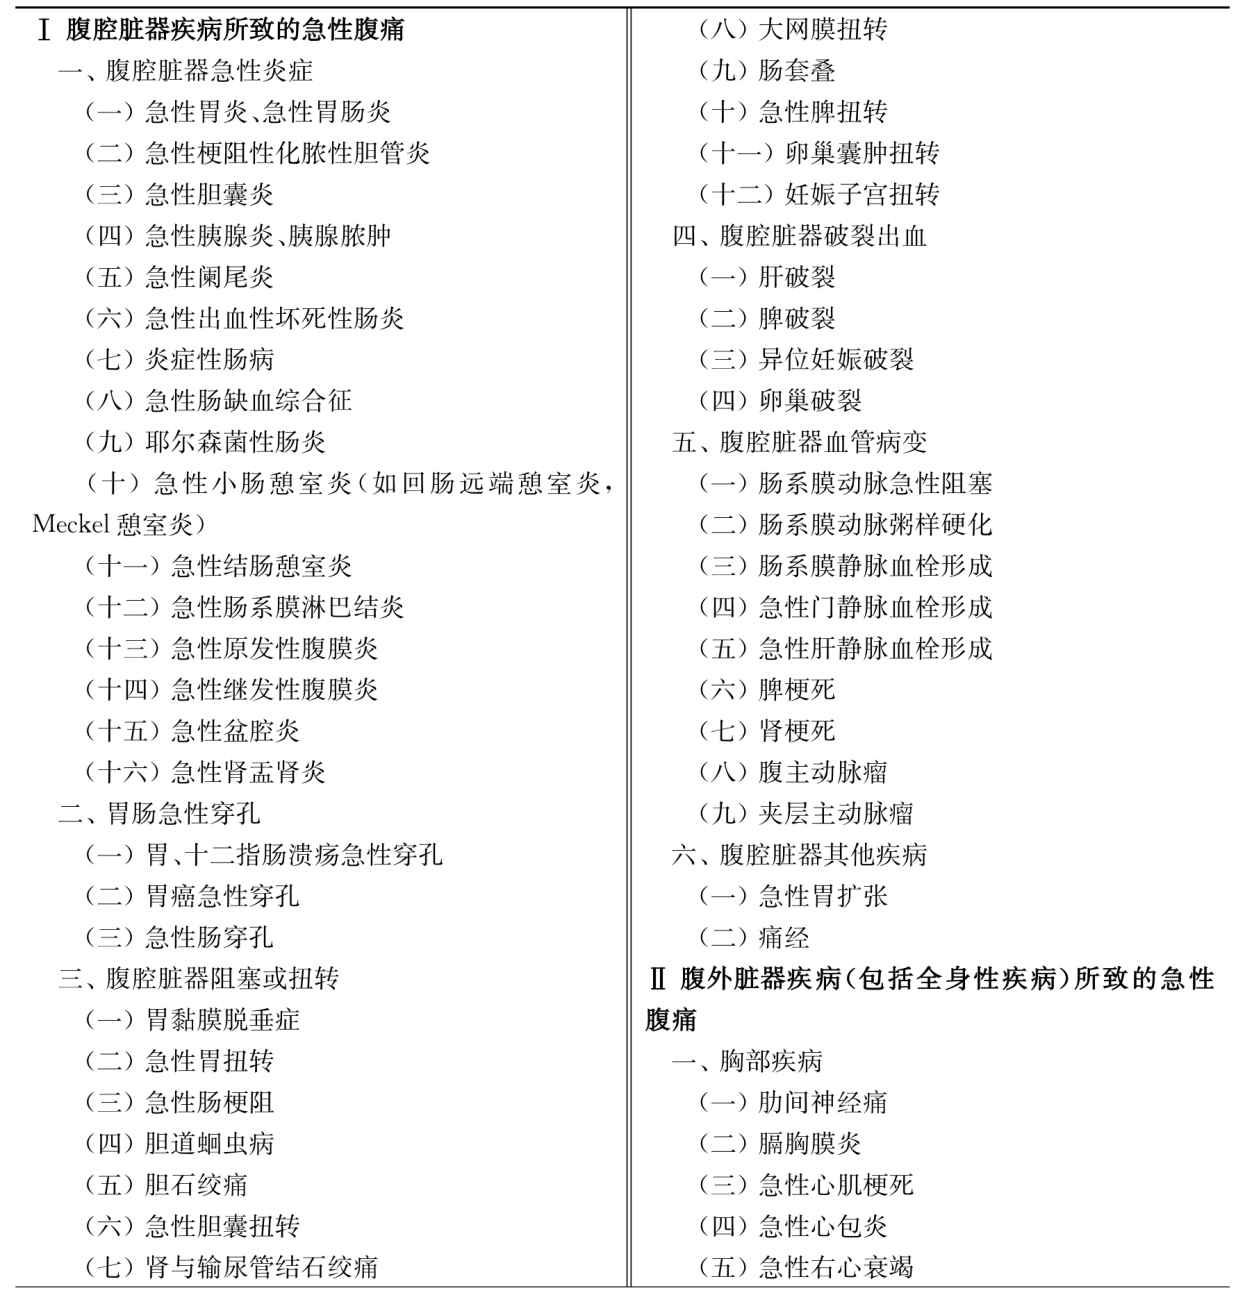
\includegraphics[width=\textwidth,height=\textheight,keepaspectratio]{./images/Image00141.jpg}\\
 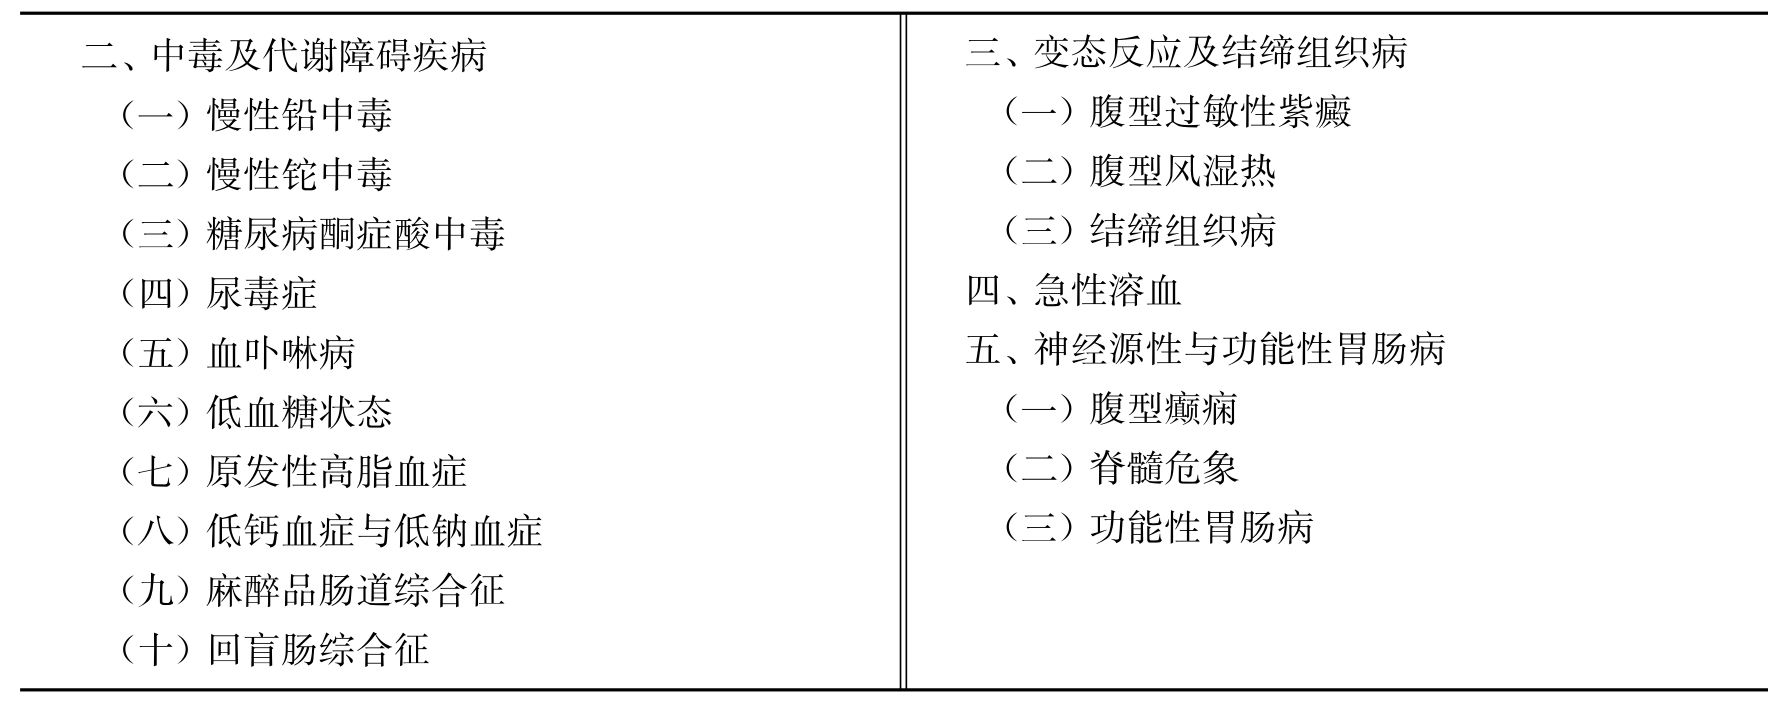
\includegraphics[width=\textwidth,height=\textheight,keepaspectratio]{./images/Image00142.jpg}
 \end{longtable}

\protect\hypertarget{text00194.html}{}{}

\section{78 腹腔脏器疾病}

\subsection{78.1 腹腔脏器急性炎症性疾病}

局限性或弥漫性腹部压痛,发热,或伴有恶寒或寒战,血象白细胞增多与左移,提示腹腔器官急性炎症性病变的可能性。

\subsubsection{一、急性胃炎及急性胃肠炎}

急性胃炎可仅表现为上腹部疼痛,伴有恶心、呕吐。如出现腹泻,称为急性胃肠炎。肠炎多表现为脐周或全腹部广泛或不定位疼痛,性质多为阵发性绞痛,也有部分患者表现为持续性胀痛或隐痛,尤其是在病程的中后期。部分患者(尤其是应激、药物等所致的急性胃肠炎患者)可出现消化道出血。急性胃肠炎可为感染性(可为各种病原体感染,常见的病原体有病毒和细菌,后者更常见,而且多与进食不洁食物有关)或非感染性(如应激、药物或酗酒等),临床上以感染性急性胃肠炎更多见。急性胃肠炎的重要特征是去除病因或治疗后病情常于短期内好转。

散发性急性胃肠炎患者如就诊时未发生腹泻,而以剧烈的腹痛为主诉,可能误诊为其他急腹症。有时急性肠炎患者以急性右下腹痛起病,伴有触痛,可被误诊为急性阑尾炎,但重复检查右下腹并无固定压痛点、肠鸣音亢进,腹痛为阵发性,与一般的急性阑尾炎不符。急性阑尾炎也可有腹泻,但程度较轻,与急性胃肠炎的水样泻不同。急性阑尾炎有时因盆腔腹膜炎刺激直肠引起排便次数增多,但粪便量不多或仅有少许黏液,与急性胃肠炎有别。偶尔急性胃肠炎在X线透视下有肠液平面,可被误诊为不完全性肠梗阻,须继续观察才能鉴别。值得注意的是,有些慢性疾病,如暴发型炎症性肠病等,也可能以急性腹痛为首发症状而被误诊,因此对于反复急性腹痛发作或病程迁延者,宜排除其他疾病(参见慢性腹痛部分)。有些急腹症也可被误诊为“急性胃炎”,其中最多是急性阑尾炎,依次为胆道蛔虫病、急性胰腺炎、胆囊炎、胆石症等。如注意这些急腹症的临床特点,细致的动态观察,可避免误诊。急性胃炎在呕吐之后腹痛往往减轻,病情常于短期内好转,而上述的急腹症有关急性胃肠炎的鉴别诊断参见第73节。

\subsubsection{二、急性胆管炎、急性胆管炎及急性梗阻性化脓性胆管炎}

急性胆管炎表现为胆道感染的Charcot三联症:右上腹痛、寒战高热和黄疸;急性梗阻性化脓性胆管炎除具备Charcot三联症外,常伴有休克和神经中枢系统受抑制的表现(即Reynolds五联症)。本病血象白细胞增多,以中性粒细胞为主,常伴有核左移等,肝功能检查常有肝酶学和胆红素升高(参见第106.2节)。

\subsubsection{三、急性胆囊炎}

据国内文献报道,胆囊炎与胆石症发病率占急性腹部外科疾病的第二位。急性胆囊炎多见于女性,发病年龄以20~40岁最多。引起急性胆囊炎的细菌以革兰氏阴性菌,特别是大肠杆菌为最多,其次是链球菌、葡萄球菌等。急性胆囊炎主要的临床表现是寒战、发热、恶心、呕吐、胀气与右上腹痛,40\%~50\%患者可出现黄疸,但如不累及胆管系统,可无黄疸。疼痛一般位于右上腹部胆囊区,程度较剧烈而持久,常有间歇性加剧,可向右肩胛区放射。如伴有结石梗阻则疼痛程度更为严重。腹痛常于饱餐尤其进食较多脂肪之后发作。用左手拇指放于肋缘下胆囊处,略加压力,嘱患者深吸气,患者感到疼痛加剧及有突然呼吸屏息现象,即Murphy征,是一个有重要诊断意义的体征。患者右上腹有明显的压痛与肌强直。约1/3患者可在右肋缘下触及椭圆形肿大的胆囊。白细胞总数增多与核左移现象。胆囊平片有时可发现结石,对诊断有帮助。B超发现肿大和充满积液的胆囊和结石征象。

值得注意的是,4\%~8\%急性胆囊炎患者为急性非结石性胆囊炎,临床表现虽与急性结石性胆囊炎相似,但本病发生于严重创伤、烧伤或手术后,或继发于其他危重疾病,相关的症状和体征已被原发疾病的症状和体征所掩盖,导致误诊和延误治疗的发生率可高达50\%。提高对本病的认识和警惕性,对右上腹部压痛及腹膜刺激征或扪及肿大触痛的胆囊者,宜早期行B超、CT等检查,结合血常规、肝功能生化学检查结果进行分析。

急性胆囊炎可误诊为高位急性阑尾炎。前者的疼痛在右上腹部,而后者在右腰部或右下腹上方,且急性胆囊炎在肋缘下可触及肿大的胆囊,并有胆囊触痛征及Murphy征,可与阑尾炎鉴别。十二指肠球部溃疡将发生穿孔而引起溃疡周围炎时,可类似急性胆囊炎并发局限性腹膜炎,但前者往往有典型节律性胃痛史,也可能有上消化道出血史,若无反指征时作胃、十二指肠镜或X线钡餐检查有助于鉴别。黄疸型病毒性肝炎有时可出现胆囊炎样绞痛,易与此病混淆,但前者常有食欲不振、疲乏无力等症状,体检无胆囊触痛征或Murphy征,白细胞一般不增加,而淋巴细胞相对增加,且转氨酶活性明显升高,不难与急性胆囊炎相区别。其他应排除腹腔内外的其他疾病,如急性胰腺炎、肝脓肿、结肠肝曲憩室穿孔及右侧肺炎或胸膜炎等。

\subsubsection{四、急性胰腺炎}

急性胰腺炎在临床上比较常见,可区分为两种类型:轻症,病情较轻,胰腺水肿,无明显的出血坏死和渗出,不伴有胰腺本身或全身并发症;重症,病情严重,常伴有胰腺并发症(如胰腺出血、坏死,胰腺囊肿或脓肿)和(或)全身其他并发症。轻症型临床上最多见,占急性胰腺炎病例的80\%~90\%,一般采用内科保守疗法。急性胰腺炎发病急,主要与暴饮暴食(尤其是过多进食高脂食物)、饮酒、胆道蛔虫及精神激动等诱发因素有关。其主要的临床表现是急性上腹痛,多位于中上腹部,其次是左上腹、右上腹或脐部,疼痛以仰卧位为甚,坐位和向前倾可减轻,多呈持续性钝痛、钻痛或绞痛,常阵发性加剧,并向左腰背部放射(见图\ref{fig25-3})。常伴有中低度发热、恶心、呕吐,呕吐每于腹痛发生不久即出现,常甚剧烈,但不持久,这是急性胰腺炎的特点之一。疼痛一般较剧烈,严重者(重症)可发生休克。重症急性胰腺炎与胃肠穿孔均可在疾病早期即出现急性腹痛,伴休克,此时宜进行细致鉴别。腹部检查可发现中上腹或左上腹压痛、反跳痛与肌紧张。由于胰腺位于胃部之后,炎症处于深部,通常只引起轻度肌紧张,不致达到板状硬的程度;消化性溃疡急性穿孔,早期腹壁紧张即达到板状硬的程度。但须注意,少数急性胰腺炎病例可出现腹壁板状硬,有明显的压痛与反跳痛,以及移动性浊音,难与消化性溃疡急性穿孔鉴别,但通常可根据前者有血、尿淀粉酶升高,而后者常有肝浊音界缩小或消失、膈下气影等而鉴别之。少数患者以全腹痛开始,随而转至右下腹痛,阑尾压痛点有明显压痛与反跳痛,类似急性阑尾炎。血清与尿淀粉酶测定,对诊断急性胰腺炎有决定性意义,血清淀粉酶在发病后6~12小时开始增高,而尿淀粉酶增高略迟。血清淀粉酶超过正常值应怀疑本病的可能性,升高至正常高限值三倍时有重要诊断价值。其他急腹症如胃、十二指肠溃疡穿孔、肠梗阻、胆囊炎、胆石症等,血清淀粉酶虽也可增高,但很少超过正常高限值三倍。血清淀粉酶一般在发病后24~48小时内最高,2~5天内下降复常;尿淀粉酶在发病后12~24小时开始升高,24~48小时内最高,下降也较晚,但较不规则,且不够灵敏,易受尿量等因素的影响,不如血清检验的可靠。腹水淀粉酶增高也有参考价值。高度怀疑急性胰腺炎的患者如淀粉酶数值不高,宜反复测定,以免漏诊。急性腹痛伴低钙血症性手足搐搦症,如无慢性肾脏病存在,也支持急性胰腺炎。在较晚期病例,血清脂酶测定超过15U/L,对诊断也有帮助,特异性较高,而且血清脂肪酶常在起病24~72小时升高。持续7~10天,对就诊较晚的急性胰腺炎患者的诊断更有帮助。

急性胰腺炎患者如同时有明显的腹膜炎体征与血性腹水(包括腹水淀粉酶升高),是确定胰腺实质坏死出血的可靠征象。CT(平扫加增强)对早期诊断胰腺炎及判断有无胰腺出血坏死、有无囊肿、脓肿等有较高的诊断价值。

胰腺脓肿是急性胰腺炎的严重并发症,临床上相对少见。脓肿常在急性胰腺炎后4~6天形成,少数可因继发感染程度较轻而延至起病后2~4周。急性胰腺炎后并发胰腺脓肿的发病率常与胰腺坏死的程度和范围有关。急性胰腺炎在常规治疗过程中病情突然恶化,白细胞日趋升高与中性粒细胞核左移加重,对积极治疗效应差,并有上腹痛、压痛和脓毒血症三联症,是脓肿形成的表现。血培养可阳性。B超有一定的参考价值,CT(平扫加增强)有较高诊断价值和评估胰腺炎严重程度的价值。少数诊断不明,或合并有外科手术指征者,可考虑手术探查明确诊断。急性胰腺炎诊断时应注意:①必须强调临床表现在诊断急性胰腺炎中的重要地位。持续性中上痛、血清淀粉酶增高、影像学改变,排除其他疾病,可以诊断本病;②临床上不再应用“中度急性胰腺炎”或“重症急性胰腺炎倾向”;③临床上应注意一部分急性胰腺炎患者从“轻症急性胰腺炎”转化为“重症急性胰腺炎”可能。因此,必须对病情作动态观察。对于胰腺炎严重程度分级,除CT扫描评估外,尚可用Ranson指标、APACHE-Ⅱ指标,以及其他有价值的判别指标,如体重指数超过28kg/m\textsuperscript{2}
;胸膜渗出,尤其是双侧胸腔积液;72小时后CRP>150mg/L,并持续增高等均为临床上有价值的严重度评估指标(表\ref{tab25-3})。\footnote{A~C级:临床上为轻型急性胰腺炎;D、E级:临床上为重症急性胰腺炎}

\begin{table}[htbp]
\centering
\caption{根据CT扫描(平扫加增强CT)时胰腺炎症的严重程度分级}
\label{tab25-3}
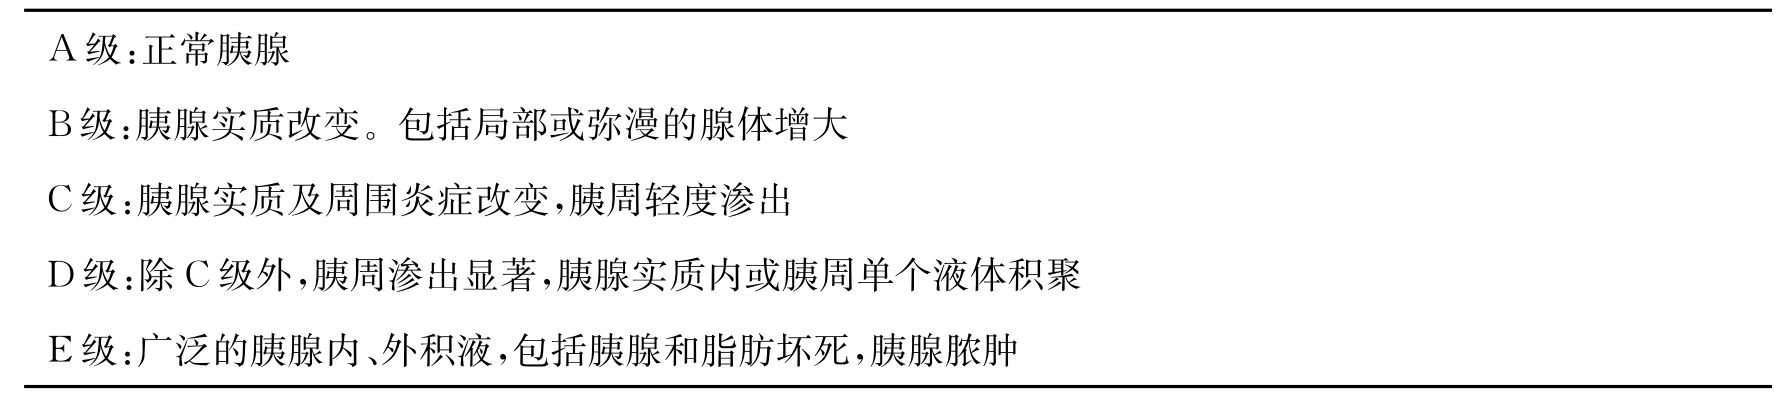
\includegraphics[width=5.95833in,height=1.32292in]{./images/Image00143.jpg}
\end{table}


值得注意的是,老年人急性胰腺炎具有临床表现不典型、病情重、并存症多的特点,有报道称,老年人急性胰腺炎的诱因主要为胆石症(81/122例,66.3\%),主要临床表现为腹痛、发热,其中2例因腹痛症状轻微,血淀粉酶升高不明显而漏诊,尸检证实为急性胰腺坏死;重症胰腺炎31例(25.4\%),重症胰腺炎突出表现为呼吸功能不全22例(70.9\%),休克7例(22.5\%),肾功能不全5例(16.1\%);并存症主要为心、脑、肺疾病及糖尿病;死亡6例,病死率为4.9\%,死因主要为休克。

\subsubsection{五、急性阑尾炎}

急性阑尾炎是误诊较多的急腹症,尤其是部分轻症或不典型患者(后者常与阑尾位置变异有关),其症状是由于腹膜炎症刺激与毒血症所引起,主要表现为:脐周或中上腹部疼痛,伴有恶心、呕吐;腹痛转移或集中在右下腹;右下腹有明显压痛;体温升高;白细胞增高与核左移现象。一般来说,若先发热或先呕吐,然后出现腹痛的患者,不符合急性阑尾炎。食欲不振也是常见的症状。一向健康的人,突然食欲不振,并有上腹疼痛,应注意此病的可能。早期可发现右下腹呼吸运动与腹壁反射减弱或消失。血象在鉴别诊断上也值得重视,此病表现为中性粒细胞增多与核左移、嗜酸性粒细胞减少或消失。若白细胞总数与分类正常,且嗜酸性粒细胞计数正常或增多时,则不支持急性阑尾炎。但须注意,在病程早期白细胞可以尚未发生改变。

急性阑尾炎的诊断主要根据上述症状,以及阑尾压痛点(麦氏点)有明显压痛、反跳痛,右下腹肌紧张,挤压左下腹可引起右下腹疼痛(即结肠充气试验)等体征做出。后位阑尾炎时,将患者右下肢向后过度伸展时,可使右下腹疼痛加剧(即腰大肌征阳性)。直肠指检通常右上方有压痛。值得注意的是右下腹肌紧张不一定存在,尤其位于骨盆内未穿孔的阑尾炎不致引起腹肌紧张。全身衰弱、老年人、孕妇或小儿等,也可不出现腹肌紧张,但患侧与健侧腹肌互相仔细比较,可发现有不相同的抵抗感。B超可实时显示阑尾病变位置和程度,确诊率甚高,B超诊断符合率为93.1\%。部分患者因诊断不明行结肠镜检查排除其他疾病时,发现阑尾开口有脓性分泌物有助于诊断。

回肠远端憩室炎(Meckel憩室炎)症状与急性阑尾炎酷似,鉴别不容易,但其疼痛与压痛点较高而更靠近脐部或在中下腹偏左,腹部症状与体征的局限化较早;腹部CT等有助于鉴别,部分患者须手术方能鉴别。

阑尾梗阻与急性阑尾炎的症状非常近似,手术前难以区别,但细心检查仍可发现有不同之处。阑尾梗阻的症状并不如急性阑尾炎随时间的推移而迅速加重;腹痛常直接在右下腹出现,无转移性痛;腹肌紧张与肛门指诊触痛均较少见。阑尾梗阻的确诊须靠手术及病理检查。切除阑尾后症状即消失。

阑尾蛔虫病临床表现与一般急性阑尾炎相似,但也有其特点。在蛔虫钻入阑尾的初期,感染症状尚未明显,表现为阵发性右下腹剧烈疼痛,发作过后,即感轻松。小儿患者发病前多有服驱蛔药史。早期症状重而体征轻微,仅在阑尾压痛点(麦氏点)附近有压痛,或可在右下腹触及有压痛的条索状物。晚期阑尾发生急性炎症或穿孔,则难与一般急性阑尾炎鉴别。

阑尾类癌是阑尾最常见的肿瘤,大多数无症状,经手术或尸检时偶然发现。2/3病例为女性。由于大多数类癌位于阑尾的尖部,单个存在而细小,很少引起症状。如增大而发生机械性梗阻,可表现为急性阑尾炎的病征。

部分局限于回肠末端或右半结肠的疾病,如克罗恩病、肠结核、白塞病、以及阿米巴、肠伤寒、血吸虫病等,有些患者临床表现与急性阑尾炎大致相似。由于此病发病率和临床知晓率均较低,不引人注意,故大都术前误诊为急性阑尾炎。此病有以下几个特点可供与急性阑尾炎鉴别参考:①急性右下腹痛同时伴有多次腹泻或带有黏液的稀便、间有血便;②局部压痛不明显或压痛部位比较高,多在阑尾压痛点稍上方或其有侧脐水平线之上;③在发病24~36小时内,右下腹可出现痛性肿块。选择性钡剂灌肠或结肠镜可发现回肠末端或右半结肠病灶。

女性急性阑尾炎患者还须注意与急性右侧输卵管炎、右侧异位妊娠破裂、卵巢囊肿扭转、卵巢黄体或滤泡破裂等相鉴别。急性输卵管炎压痛点较低,在阑尾压痛点下方或耻骨上区,阴道有分泌物,阴道检查宫颈有明显触痛;异位妊娠破裂有停经史、腹腔内积血与阴道流血,甚至休克的表现,可与急性阑尾炎相区别。B超或腹部CT检查有助于明确诊断。

此外,急性阑尾炎在临床上尚需与低位急性胆囊炎、胃十二指肠溃疡穿孔、急性局限性肠炎、右侧输尿管结石、急性肠系膜淋巴结炎等相鉴别(参考本章有关部分)。

下列一些特别情况的急性阑尾炎,临床表现常不典型,在诊断上须特别注意。

\paragraph{(一)老年人急性阑尾炎}

症状与体征不典型或轻微,容易误诊。腹痛往往只限于上腹部或脐周。少数患者甚至无自觉腹痛。恶心、呕吐也较少。无发热者也不少见,但体温正常而脉率显著加快,对诊断有提示作用。恶寒虽不多见,但有一定的诊断意义。腹部压痛(最多位于右下腹)是主要的病征,大多有明显的反跳痛。白细胞总数不增加者也不少见,甚至阑尾炎穿孔而白细胞总数也可不增多,但往往分类计数中性粒细胞增多与有明显核左移现象,嗜酸性粒细胞及淋巴细胞显著减少,老年人急性阑尾炎并发早期穿孔的发病率高,不应强求典型征象,凡可疑病例,应密切观察,反复检查,以免延误诊断。

\paragraph{(二)妊娠期急性阑尾炎}

妊娠期急性阑尾炎可发生在妊娠任何期间,多发生于21~40岁之间的经产妇。其临床表现不典型,诊断往往发生困难。诊断困难的原因是:①在妊娠期间,阑尾常随子宫的增大而被推向上外方,致阑尾痛区及压痛点有所改变,逐渐移至脐旁和脐部上外方;②增大的子宫可将阑尾遮盖,阑尾的炎症不波及前腹壁腹膜;③在多次妊娠时,腹壁松弛,虽腹膜有炎症性刺激,腹肌紧张与腹壁压痛也可不显著,甚或无肌紧张与压痛;④妊娠期间可有生理性白细胞增多、体温稍高、脉搏稍快等表现。上述各种情况可造成诊断上的困难。

在临床上如孕妇发生持续的急性腹痛,伴恶心、呕吐、发热,或兼有右腹部局限性压痛者,应考虑急性阑尾炎的可能。既往有右下腹疼痛史,对诊断有帮助,50\%妊娠期急性阑尾炎患者,有右下腹痛既往史。体检常可发现阑尾痛点或其上方有压痛、反跳痛与不同程度的肌紧张,特别是嘱孕妇卧向左侧,子宫向左移位时,发现右侧腹肌稍紧张,有时并有压痛与反跳痛,有诊断意义。

\paragraph{(三)血吸虫病并发急性阑尾炎}

血吸虫病并发急性阑尾炎,过去在严重流行区发病率很高。血吸虫卵沉着于阑尾壁内,引起纤维性变,使阑尾腔狭窄和血运减少,易于发生急性炎症。急性炎症发生后且易于早期穿孔,有些患者甚至发病4小时后已发生阑尾穿孔,因而65\%~70\%患者就诊时已并发腹膜炎。白细胞总数在阑尾穿孔也常无著升高。血吸虫病患者突然发生右下腹痛时,应注意此病的可能,须严密观察及时作出诊断与处理。有经手术后病理检查确诊阑尾血吸虫病并发急性阑尾炎的275例患者临床回顾性分析发现,男性176例,女性99例;年龄最大75岁,最小6岁,平均36岁,占同期急性阑尾炎的35.9\%(275/765),临床表现均有不同程度右下腹压痛、反跳痛、肌紧张。93例有全腹压痛、反跳痛、肌紧张。所有患者均来自血吸虫病疫区,有血吸虫病史41例。全组患者转移性右下腹痛者198例,发热237例,呕吐182例。86例有肝左叶增大。实验室检查:血常规均升高,其中嗜酸性粒细胞增高者58例,占21.0\%。

\subsubsection{六、急性出血性坏死性肠炎}

急性出血性坏死性肠炎(acute hemorrhagic necrotizing
enteritis)是与C型产气荚膜梭菌感染有联系的一种急性肠炎,急性出血性坏死性肠炎病变主要在小肠,病理改变以肠壁出血坏死为特征。其主要临床表现为腹痛、便血、发热、呕吐和腹胀。严重者可有休克、肠麻痹等中毒症状和肠穿孔等并发症。此病的特点之一是突然发生的急性腹痛,疼痛多位于左上腹或左中腹部,也可位于脐部,偶尔扩散至全腹,须注意与急性胃肠炎、急性胰腺炎等相鉴别。急性出血性坏死性肠炎与急性阑尾炎比较,前者病情重,进展更快,有时伴有血便,腹部体征常不固定在麦氏点,肠鸣音早期增强,随后减弱消失。①血常规:外周血白细胞增多,甚至高达40.0×10\textsuperscript{9}
/L以上,以中性粒细胞增多为主,常有核左移。红细胞及血红蛋白常降低。②粪便检查:外观呈暗红或鲜红色,或隐血试验强阳性,镜下见大量红细胞,偶见脱落的肠系膜,可有少量或中等量脓细胞。还可做细菌涂片和培养。生化学检查发现血肌酐和尿素氮升高有助于诊断。③X线检查:腹部平片可显示肠麻痹或轻、中度肠扩张。钡剂灌肠检查可见肠壁增厚,显著水肿,结肠袋消失。在部分病例尚可见到肠壁间有气体,此征象为部分肠壁坏死,结肠细菌侵入所引起;或可见到溃疡或息肉样病变和僵直。部分病例尚可出现肠痉挛、狭窄和肠壁囊样积气。诊断主要根据临床症状。突然腹痛、腹泻、便血及呕吐,伴中等度发热,或突然腹痛后出现休克症状,特别是患者排有腥臭味洗肉水样便而没有明显里急后重时,应考虑急性出血性坏死性肠炎的可能。腹部X线平片有助于诊断。

\subsubsection{七、炎症性肠病及白塞病}

炎症性肠病包括溃疡性结肠炎(UC)和克罗恩病(CD)。暴发型溃疡性结肠炎患者可出现急性腹痛,常伴有全身症状(如发热、贫血、消瘦、乏力等)或肠外表现(皮肤、关节、眼部及肝胆等脏器的病变),常伴有腹泻黏液脓血便。克罗恩病多见于脐周或右下腹痛,常被误诊为急性阑尾炎而行手术治疗(参见第24章)。

\subsubsection{八、急性肠缺血综合征}

急性肠缺血综合征(AMI)是由各种原因引起肠道供血不足而发生的综合征,包括肠系膜上动脉栓塞、急性肠系膜上动脉血栓形成、非肠系膜血管阻塞性肠梗阻、肠系膜上静脉血栓形成、缺血性结肠炎以及其他原因的肠道血管病变所致的肠道缺血性疾病等。根据缺血的程度分为梗死性和非梗死性缺血性肠病,又以前者的病情更为凶险。有关缺血性肠病患病率的流行病学资料尚不多见。国外研究表明,急诊监护病房每1000例患者中就有1例AMI患者;危险因素静息状态下胃肠道动脉血流量占心排血量的10\%,而运动或进餐后消化道血流量变化较大。引起本病的要病理基础是局部血管病变、血流量不足或血液的高凝状态。危险因素主要有:心力衰竭、心律失常、心房颤动、各种原因所致的休克、动脉血栓形成、机械性肠梗阻等。医源性因素有动脉瘤切除术、主动脉手术、冠状动脉搭桥术、肠切除术、肠镜、钡灌肠、妇科手术等;药物因素有可卡因、达那唑、地高辛、雌激素、苯异丙胺、利尿剂、非甾体消炎药等,均可导致老年人缺血性肠病发生。约80\%患有肠系膜动脉阻塞是由动脉粥样硬化和风湿性心脏病引起的,其次是血管造影后动脉粥样硬化斑块脱落所致,老年人出现不明原因的腹痛、血便、腹泻或腹部急腹症表现者应警惕结肠缺血的可能,尤其是合并慢性心瓣膜病伴心房颤动、亚急性细菌性心内膜炎、高血压动脉硬化、肝硬化门脉高压或腹部手术后等情况下发生急性腹痛时,需考虑腹腔内脏器血管发生痉挛、梗死或血栓形成导致缺血性肠病的可能性。

临床表现无特异性,首发症状常为难以忍受的剧烈腹痛,动脉缺血起病急骤,静脉缺血起病徐缓,常有数日的非特异性前驱症状,解痉剂及阿片类强烈止痛药效果差,早期腹痛与体征不符。典型急性缺血性肠病的三联症:剧烈上腹痛或脐周痛而无相应的体征,器质性心脏病合并心房颤动,胃肠道排空障碍。急性缺血性肠病的特点之一是突然发生的急性剧烈腹痛,疼痛多位于左上腹或左中腹部,也可位于脐部,偶尔扩散至全腹,伴频繁呕吐和腹泻为主要症状,约75\%患者大便潜血阳性,15\%患者可伴有血便;部分患者可出现肠梗阻;部分重症患者可出现溃疡及穿孔。本病诊断较为困难,主要根据急性严重腹痛,症状和体征严重程度不成比例,体征常不明显;如临床观察中如出现腹部压痛逐渐加重、反跳痛及肌紧张等,则为肠缺血进行性加重的表现,强烈提示已发生肠坏死。实验室检查无特异性,外周血白细胞和血尿淀粉酶可升高。腹部X线检查可见“指压痕”征、黏膜下肌层或浆膜下气囊征。多普勒超声、MRI和选择性肠系膜血管造影等对腹腔血管病变诊断意义较大。彩色多普勒超声可显示肠系膜血管的情况,测定血流速度、血流量和截面积。CT检查可见肠壁及血管内栓子,显示静脉侧支循环及肠壁缺血节段的位置,对肠系膜缺血的确诊率达66.7\%,肠系膜上动脉不显影、腔内充盈缺损;肠黏膜组织病理学检查以缺血性改变为主要特点,如伴有血管炎、血栓形成及血管栓塞病变者即可确诊。动脉造影有助于鉴别诊断,血管造影可显示病变区域血管狭窄或中断,以及充盈缺损、充盈缓慢、不显影等相应的影像学改变。对疑似病例应尽早行血管造影,选择性肠系膜血管造影是诊断肠系膜动脉缺血最可靠的方法。由于本病临床表现和辅助检查无特异性,临床医师认识不足、警惕性不高,须注意与急性胃肠炎、急性胰腺炎等相鉴别,特别是急性胰腺炎患者,由于使用生长抑素类药物,该药可收缩内脏小动脉,加重肠缺血,影响患者预后,此时应高度注意是否合并缺血性肠病。但此类疾病中常伴有排血便等,早期肠鸣音常活跃或亢进,但很快出现肠鸣音减弱或消失,血管超声检查对较大血管的病变有一定的帮助,而选择性肠系膜血管造影对肠系膜动脉病变有一定的参考价值,造影显示病变血管阻塞或痉挛。本病病情发展迅速,一般情况迅速恶化,出现肠麻痹、弥漫性腹膜炎、血性腹水等表现,全身中毒症状明显,如不及时治疗,很快出现感染性休克,病死率高。

文献报道,梗死性缺血性肠病26例,其中男15例,女11例,年龄36~84岁,平均68.6岁。合并高血压、冠状动脉硬化性心脏病者10例,心瓣膜病6例,同时伴心房纤颤8例,脑梗死3例,有肝硬化者7例,合并腹腔内感染性疾病2例。临床表现均有剧烈腹痛,伴恶心24例,呕吐12例,腹泻9例,便血10例。早期腹肌软,压痛点不固定,肠鸣音活跃或亢进,全部病例分别于1~3天出现肠麻痹、弥漫性腹膜炎、血性腹水及全身中毒症状等。实验室检查血性腹水占80.8\%,外周血白细胞升高占84.6\%,血尿淀粉酶升高占53.9\%。彩色多普勒超声阳性率为50.0\%,CT阳性率为67\%,肠系膜上动脉造影阳性率为80.0\%。

\subsubsection{九、耶尔森菌性肠炎}

在北欧、北美洲均报告有由耶尔森菌(Yersinia
enterocolitica)引起的急性末段回肠炎和结肠炎。40\%病例有类似急性阑尾炎的表现,以儿童与少年为多。80\%病例则以腹痛与腹泻为主诉,表现为急性肠炎。病理组织活检为肠系膜淋巴结炎与急性末段回肠炎和结肠炎。全消化道X线气钡双重造影或钡灌肠检查及电子结肠镜检查所见为末段回肠黏膜及结肠黏膜粗糙与不规则或结节样变、溃疡征象等。诊断主要根据进食被污染的水源或食物,典型临床表现和大便培养证明此菌的存在。

\subsubsection{十、回肠远端憩室炎(Meckel憩室炎)}

发病年龄以幼儿与青少年较多,男性占绝大多数。其主要临床表现为腹痛、呕吐、右下腹压痛、腹肌紧张;发热和白细胞增高,并可有肠梗阻现象。临床上与急性阑尾炎酷似,难以鉴别;此病痛点比阑尾炎更向内移,可能在中下腹或左下腹,便血比较罕见,也与阑尾炎不同。此病常有出血、穿孔等并发症。如小儿或年轻患者出现上述症状并有血便,或原因未明的急性机械性肠梗阻、又无剖腹病史者,应注意回肠远端憩室炎的可能。全消化道X线气钡双重造影,胶囊内镜和双气囊小肠镜检查有助于提高诊断率,部分患者须靠手术探查方能确定诊断。

\subsubsection{十一、急性结肠憩室炎}

结肠憩室好发于乙状结肠,患者大都为中年以上的肥胖体型者,惯常在坐位工作,有习惯性便秘。憩室急性发炎时,则有发热、白细胞增多;左下腹疼痛与压痛,故急性乙状结肠憩室炎也有左侧“急性阑尾炎”之称。炎症消退后X线气钡灌肠双重造影与电子结肠镜检可确诊。

\subsubsection{十二、急性肠系膜淋巴结炎}

此病临床上少见,可发生于任何年龄,但以8~12岁儿童较为多见,有人认为是病毒感染所致。由于肠系膜淋巴结以回肠末端最丰富,故发炎后腹痛多位于右下腹部。腹痛常随同上呼吸道感染而出现,呈持续性,常位于右下腹。部分患者可先出现脐周疼痛,随而转移至右下腹,并伴有右下腹压痛,酷似急性阑尾炎。下列几点可作为两者鉴别诊断的参考:①急性肠系膜淋巴结炎多与上呼吸道感染同时存在;②腹痛较轻;③无固定压痛点与腹肌紧张;④白细胞无显著增多;⑤急性肠系膜淋巴结炎的腹痛多于短时间内减轻或消失,而急性阑尾炎的腹痛多继续发展。因此如果观察数小时,多可得出结论。如经4~6小时观察而腹痛减轻则多属急性肠系膜淋巴结炎,如腹痛不减或反而加剧,则须按急性阑尾炎处理。据报告,两病同时存在者也不少见。近年来有报道,高频超声或腹部CT在诊断小儿急性肠系膜淋巴结炎及合并症有较好的参考价值,CT或高频超声声像图特征是(右侧中下)腹部见多枚大小不等椭圆形低回声结节(肿大淋巴结)。

\subsubsection{十三、急性原发性腹膜炎}

急性原发性腹膜炎临床上少见,患者以儿童及青少年为多。此病是血行感染引起的腹膜炎症,致病菌以溶血性链球菌最多,其次是肺炎双球菌和大肠杆菌。常在上呼吸道感染、丹毒、猩红热等感染过程中发生,也可发生在肝硬化、晚期血吸虫病及肾病综合征等合并腹水的基础上,但也可无明显诱因。多数患者有营养不良或抵抗力较差。其主要临床症状是急性腹痛、寒战、发热、恶心、呕吐。腹痛往往是突然发生,一般无特别明显的部位,可遍及全腹,疼痛多较剧烈。发病初期常伴有腹泻,排水样便,甚至出现脱水现象。晚期由于肠麻痹而呈便秘。此外也常有尿频、尿急等膀胱激惹症状。体检可发现全腹有明显压痛,腹肌紧张,反跳痛。但若发生在肝硬化、晚期血吸虫病及肾病综合征等合并腹水的基础上可较轻,常表现为腹水增多、全身状况恶化等,腹膜刺激征也不明显。急性原发性腹膜炎与继发性腹膜炎临床表现非常相似,但后者多先有急性阑尾炎或消化性溃疡病病史,腹痛发生一段时间后才出现发热及其他毒血症症状,腹部腹膜刺激征较明显。急性原发性腹膜炎早期即发热,毒血症症状明显,腹部体征却不及继发性腹膜炎明显。此病在鉴别诊断上又须与渗出性结核性腹膜炎鉴别,后者发病日期不明确,进展较缓,毒血症及腹膜刺激征较轻,腹水检查以淋巴细胞占优势,可发现结核杆菌而无其他细菌。原发性腹膜炎的诊断主要根据腹水白细胞计数及多形核细胞(PMN)计数(WBC>500×10\textsuperscript{9}
/L,PMN>50\%或250×10\textsuperscript{9}
/L)和细菌学培养阳性,结合上述病史、症状与体征,排除继发性腹膜炎与结核性腹膜炎而确定之。

各种原因所致的失代偿期肝硬化并发急性原发性腹膜炎时,细菌除由体循环进入腹腔外,也可从门静脉系统直接侵入腹腔。起病较缓,腹痛轻重不等,多呈持续性胀痛或阵发性绞痛,腹膜刺激征也不明显,又因患者原有脾功能亢进,外周血象白细胞增多也可不明显,因此容易误诊。临床上遇到晚期肝硬化患者有原因未明的腹痛、发热、腹水增多,血象白细胞总数稍增高与核左移、腹水属炎性渗出液时,应考虑此病的可能,宜反复作腹水常规涂片及细菌培养检查。腹水混浊多呈浅黄色,常含有大量白细胞,培养可发现致病菌,大多是大肠杆菌。诊断主要根据腹水白细胞计数及多形核细胞(PMN)计数(WBC>500×10\textsuperscript{9}
/L,PMN>50\%或250× 10\textsuperscript{9}
/L)和细菌学培养阳性。值得注意的是,肝硬化患者合并结核性腹膜炎的发生率近年报道有所升高。

\subsubsection{十四、急性继发性腹膜炎}

继发性腹膜炎是腹腔器官病变直接感染或刺激腹膜所致的急性炎症,常见的病因归纳如下:阑尾穿孔,胃、肠溃疡或憩室穿孔,胆囊或胆道穿破,肝或脾脓肿破裂,绞窄性肠梗阻、肠扭转或肠套叠所致的肠坏死,外伤感染等。

腹痛是继发性腹膜炎最早的症状,呈持续性剧痛,胃、十二指肠溃疡穿孔时最为剧烈,而阿米巴性肝脓肿破裂时一般较轻,腹痛多由原发病变部位开始,以后可局限于该处或弥漫全腹,伴有恶心、呕吐。主要腹部体征是腹肌紧张或呈板状硬,以胃肠穿孔时最为明显。腹部压痛与反跳痛在原发病变部位尤为显著。如出现发热、脉快而弱、腹胀、肠麻痹等症状以及白细胞增多,往往提示晚期而严重的情况。

临床上有上述原发病的患者,出现急性持续剧烈腹痛、呻吟而又不敢多动、腹式呼吸与腹壁反射减弱或消失、腹肌紧张或板硬、腹部压痛与反跳痛、肠鸣音高度减弱或消失,临床上便可诊断为继发性腹膜炎。

老年人急性腹膜炎:由于机体对感染反应低下,故具有以下特点:①腹膜炎患者炎症反应不明显,约2/3左右患者可无腹肌紧张与反跳痛;②1/3患者体温可正常,甚至出现体温不升;③脉搏可不增快;④白细胞总数可不增多,甚至降低,但有明显的核左移现象。多数患者以显著的腹痛为主诉,是提示此病诊断的重要线索。老年病者有绞窄性肠梗阻、急性阑尾炎、活动性胃、十二指肠溃疡、急性胆囊炎等现病史,突然发生持续的广泛性腹痛与腹膜刺激征,肠鸣音消失,排气停止,则提示并发急性腹膜炎。血象白细胞计数虽可不增多,但分类计数中性粒细胞增多常有明星的核左移,提示重度炎症性病变。老年人急性腹膜炎并发感染中毒性休克与肾功能不全者也较多。

阿米巴性腹膜炎是较少见的疾病,但由于对此病的警惕性不高,以致未能及时诊断或误诊者亦有时见之。此病的病死率较高,肠穿孔较肝脓肿破裂更为严重。患者有未彻底治愈的肠或肝阿米巴病,而突然出现腹痛与腹膜刺激征,须首先考虑此病。腹膜刺激征以右上腹为重,而下腹部较轻,是推测肝脓肿向腹腔穿破的有力佐证。超声对诊断肝脓肿有重要的帮助。肝脓肿向腹腔穿破后,脓液多被大量腹腔渗出液所稀释,故诊断性腹腔穿刺可抽出较稀薄的棕色脓液,镜检可发现溶组织阿米巴滋养体。如无继发性感染,则脓液无恶臭,细菌培养也阴性。阿米巴病性肠穿孔的中毒衰竭症状较其他原因所致的腹膜炎严重,腹痛呈弥漫性,且以右下腹为显著,这和盲肠发病较多较重,且好发穿孔有关,在诊断上有参考价值。阿米巴病性肠穿孔的患者有阿米巴性痢疾病史和症状,且穿孔大都发生于病变的急剧发展阶段,粪中易找到阿米巴包囊或滋养体。

\subsubsection{十五、急性盆腔炎}

急性盆腔炎主要的临床症状是发热、下腹痛及白带增多。发病时即有腹痛,疼痛往往较剧烈,主要是由于输卵管、卵巢急性炎性肿胀以及盆腔腹膜发炎所致。体检可发现下腹部有明显压痛与肌紧张,部分患者肌紧张可不明显。有时与急性阑尾炎容易混淆,但此病有以下几个特点可与急性阑尾炎相鉴别:①常于月经期间、月经刚刚结束、流产或分娩之后发病;②发热及白细胞增加明显,而腹部炎症刺激征象相对地较轻;③两侧下腹均有压痛与肌紧张,且位置也较低;④白带增多;⑤肛门指检髂窝两侧均有压痛,移动子宫颈时可引起疼痛。此病多起于上行性感染,尤多继发于产后与流产后感染,病史对此病的诊断有重要意义。根据以上的病史与体征,阴道检查阴道有明显灼热感、子宫颈举痛、宫体及附件有明显压痛便可确诊。

\subsubsection{十六、急性肾盂肾炎}

急性肾盂肾炎偶尔可发生急性腹痛,类似急性胆囊炎或急性阑尾炎,须注意鉴别。

\protect\hypertarget{text00195.html}{}{}

\subsection{78.2 胃肠急性穿孔}

突然发生的腹部剧烈疼痛、伴有腹膜刺激征(板状腹、压痛与反跳痛消失),提示有胃肠急性穿孔的可能性。胃肠急性穿孔确诊主要依靠X线腹部平片提示膈下气体存在。临床上高度怀疑胃肠穿孔的不典型病例,尤其无腹部剧痛与腹壁板状硬的征象时,X线检查发现无气腹发现,可用胃管抽空胃液后注入空气300ml,则空气可自穿孔处逸出形成膈下气影,有助于胃、十二指肠溃疡穿孔的诊断。如临床表现符合胃、十二指肠溃疡急性穿孔,而注入空气后X线检查仍无穿孔的征象,应考虑手术探查。急性胃肠穿孔的诊断思路:先明确是否有穿孔,再进一步寻找穿孔的病因。

\subsubsection{一、胃、十二指肠溃疡急性穿孔}

典型胃、十二指肠溃疡急性穿孔患者,常有胃、十二指肠溃疡病史或多年反复发作的胃痛史,腹痛绝大多数突然发生,疼痛的性质很不一致,通常以持续性剧痛为多,可非常剧烈,有些患者甚至发生休克。疼痛先开始于上腹部,但迅速随着胃或十二指肠内容物由穿孔处溢流入腹腔,变为全腹的剧痛,有时以右下腹部最为剧烈,伴有明显的腹膜刺激征(板状腹、压痛及反跳痛)。消化性溃疡急性穿孔的经过可分为三个阶段:第一阶段为化学期,由于酸性胃内容物流入腹腔,刺激腹膜引起化学性炎症所致。临床表现为腹膜刺激征;约几小时后,转入第二阶段的反应性期,此期由于胃内容物已充分溢出,腹膜炎症渗出液又已中和了胃酸,患者感觉腹痛减轻,或出现欣快感,掩盖了严重的病情,应予警惕,以免延误手术治疗机会;第三阶段是化脓性感染期,但往往是临终期。

典型病例诊断大多无困难,但仍有10\%~15\%病例其临床表现颇不典型,易发生诊断错误。少数患者无典型的腹痛,且腹痛迅即消失,腹壁转为柔软,仅中上腹有轻压痛,或疼痛仅限于右下腹部,易误诊为急性阑尾炎;某些患者虽有典型胃、十二指肠溃疡穿孔的腹痛,但迅即消失,腹部仍暂时保持柔软,最后典型症状再出现,早期可误诊为胆囊炎、胆石症;个别患者,特别是衰弱的老年人,起病缓慢,初起仅有上腹部隐痛,最后疼痛又常转移至右下腹部,体征模糊,压痛部位不一,以致诊断困难。有怀疑患者宜进一步行X线腹部平片检察可发现膈下气体存在;电子胃十二指肠镜检查可发现溃疡灶,有时可见穿孔。

\subsubsection{二、胃癌急性穿孔}

胃癌急性穿孔很容易误诊,除非穿孔前胃癌的诊断已经明确。胃癌急性穿孔的临床征象与胃、十二指肠溃疡穿孔相似。下列临床表现提示胃癌存在的可能:①诊断为胃急性穿孔的患者年龄在40岁以上;②患者全身情况较差、贫血、厌食、进行性消瘦,或曾呕吐过咖啡渣样胃内容物;③穿孔前疼痛为无节律性、顽固性腹痛,进食及服碱性药物效果不佳者。

\subsubsection{三、急性肠穿孔}

急性肠穿孔可发生于肠溃疡、肠坏死或外伤,内科临床上可见于肠伤寒、慢性结肠炎、急性出血性坏死性肠炎、结肠阿米巴病等疾病。急性肠穿孔的腹痛常突然发生,一般呈持续性剧痛,常使患者不能耐受,并在深呼吸与咳嗽时加剧。疼痛范围与腹膜炎扩散的程度有关,可局限于一处或遍及全腹。患者常被迫采取仰卧位,两下肢屈曲,不愿转动。腹部检查呼吸运动显著减弱甚至消失,局部或全腹腹肌板状硬,肝浊音区缩小或消失,腹腔内有大量气体时腹部明显膨胀,肠鸣音显著减弱或消失。急性肠穿孔的诊断主要根据患者上述的病史、体征与X线检查发现有膈下游离气体。

伤寒肠穿孔:伤寒病特有的临床表现和化验检查,如持续高热、腹痛、便秘或腹泻、肝脾大、相对缓脉和白细胞减低作为与其他疾病进行鉴别的基础,在化验检查中血清肥达反应O抗体效价1∶80以上、H抗体效价1∶160以上具有诊断价值特别是从患者血骨髓、粪便中分离到伤寒杆菌具有与其他疾病鉴别的决定性意义。伤寒肠穿孔多发生于发病后第二、三周,此时伤寒一般已确诊,根据患者突然发生的腹部剧痛,以中下腹为最明显的腹肌强直与压痛,肝浊音区缩小或消失、肠鸣音消失、白细胞增高及X线检查发现气腹等,诊断一般不困难。逍遥型伤寒患者发热及毒血症症状不明显,突然发生穿孔时易误诊为胃、十二指肠溃疡穿孔、急性阑尾炎穿孔、异位妊娠破裂,特别注意须与胃、十二指肠溃疡穿孔鉴别。90\%的胃、十二指肠溃疡穿孔患者有间歇性慢性上腹痛史,穿孔发生于溃疡活动期,以冬、春季多见;伤寒肠穿孔患者无胃病史,多发生于夏秋季。另一方面,有严重毒血症的伤寒患者,常处于神志不清或昏迷状态,肠道又常有不同程度的胀气,当发生肠穿孔时,不能主诉腹痛,也无明显急腹症的征象,诊断甚为困难。如患者突然体温下降,脉搏变为细数,肠鸣音消失,腹部胀气不断增加,肝浊音区缩小或消失,中性粒细胞增多,则大致可诊断为伤寒穿孔,尤其是肠鸣音消失对伤寒肠穿孔的诊断有很大的价值;若肠鸣音很活跃,则不支持肠穿孔。X线检查多数患者可发现膈下游离气影,对穿孔的证实有决定性意义。

\protect\hypertarget{text00196.html}{}{}

\subsection{78.3 腹腔脏器阻塞或扭转}

急性发作的阵发性腹部绞痛,伴恶心、呕吐,冷汗淋漓,提示可能为腹部脏器阻塞或扭转所致的急性腹痛。胃肠扭转或梗阻常可观察到胃蠕动波或肠型,肠鸣音高亢或呈金属音。脏器扭转时可触到痛性腹部包块。胆石绞痛与胆道蛔虫病可出现黄疸。肾结石绞痛时伴有血尿。

\subsubsection{一、胃黏膜脱垂症}

胃黏膜脱垂症也可引起急性上腹痛,伴有恶心、呕吐,但一般无腹膜刺激征,较易与外科急腹症鉴别(参见第81节)。

\subsubsection{二、急性胃扭转}

急性胃扭转在临床上罕见。胃扭转是胃超过生理限度的轴性扭转。胃扭转的原因主要是由于胃韧带先天性过长而松弛;另一方面胃或膈肌病变(如胃溃疡、良性或恶性肿瘤、膈疝、胃周围炎性粘连等)对胃韧带起牵引作用,从而促使胃扭转。任何引起胃运动过快的因素,如饱食、肠炎、服用大量碳酸氢钠、分娩、外伤等均可诱发此病。

急性胃扭转的诊断根据是:①突发性上腹部间歇性或持续性疼痛,可放射至背部;②频繁干呕,并有全身衰竭情况;③左上腹可触到一紧张性痛性肿块;④胃管无法放入胃内;⑤X线腹部平片在左上腹可见两个或一个液平面,而无其他征象;⑥X线钡餐可显示胃腔(胃黏膜)扭转、变形;⑦胃镜检查发现胃腔变形、扭转。

\subsubsection{三、急性肠梗阻}

急性肠梗阻是临床上常见的急腹症,从病因方面可分为机械性、动力性(痉挛性或麻痹性)、血运性三种。从肠壁有无血运障碍又可区分为单纯性与绞窄性两种。仅有肠腔不通畅而无肠管血液供应障碍者属单纯性肠梗阻,如兼有血液供应障碍,则为绞窄性肠梗阻。肠系膜血管阻塞所致的肠梗阻,也属于绞窄性肠梗阻范围。临床上以急性机械性肠梗阻最为常见。急性机械性肠梗阻的主要原因是:粘连、外疝、扭转、套叠、蛔虫、先天性畸形、肿瘤、结核等。急性机械性肠梗阻的主要临床表现是腹部绞痛、呕吐、腹胀及便秘与排气停止。腹痛有以下特点:①急性发作,呈阵发性、波浪式绞痛,多位于脐周或下腹部;②绞痛时伴有胃肠蠕动增快,腹部检查常隐约可见腹部膨胀,出现胃肠型和蠕动波,早期常无腹膜炎样触痛,按压腹部时常反觉好受些,病变部位可有深部压痛,听诊肠鸣音高亢,有气过水音、金属音等。

机械性肠梗阻在鉴别诊断上须注意与饮食不洁、食物过敏等所致急性胃肠炎、卵巢囊肿扭转等鉴别。急性胃肠炎虽也有阵发性肠绞痛与肠鸣音增强,但肠鸣音非音调高亢,无气过水音或金属音,腹泻常明显,而呕吐较轻或不出现;卵巢囊肿扭转也有阵发性腹痛、早期呕吐,但无肠鸣音的改变,且腹部及阴道检查有张力很高、明显触痛的肿块,可与机械性肠梗阻相区别。机械性肠梗阻又须与痉挛性肠梗阻相区别。痉挛性者多为暂时性的,以0.25\%普鲁卡因溶液作两侧肾周封闭后1/2~1小时症状即缓解,而机械性肠梗阻则无效,是一种有鉴别诊断与治疗价值的方法。

怀疑肠梗阻时,首选的检查手段是X线腹部平片(立卧位对照)(一般在肠梗阻4~6小时后即可显示肠腔液气平面(值得注意的是,未见肠腔液气平面不能排除肠梗阻)。肠梗阻的诊断思路包括:①是否存在肠梗阻;②机械性肠梗阻还是动力性肠梗阻:③单纯性肠梗阻还是绞窄性肠梗阻;④高位肠梗阻还是低位肠梗阻;⑤完全性肠梗阻还是不完全性肠梗阻:⑥最后寻找肠梗阻的病因。其中明确为机械性肠梗阻后,最重要的是,必须进一步判断是单纯性抑或绞窄性。因绞窄性肠梗阻应尽可能早期进行手术,而单纯性肠梗阻则可考虑暂不作手术治疗或经充分准备后再施行手术。机械性肠梗阻的患者有下列临床征象时,应考虑是绞窄性:①腹痛发作较急而剧烈,呈持续性而有阵发性加剧,呕吐出现较早,且为持续性。②病程进展较快,早期即出现类似休克的征象,并逐渐加重,或经抗休克治疗后改善不显著。③有明显腹膜刺激征,体温、脉搏与白细胞总数有增高、增多的趋势。④血肌酐和尿素氮短时间内明显升高。⑤腹胀两侧不对称,腹部触诊或肛门指检触到有触痛的肿块。X线检查发现有持续不变单独突出胀大的肠袢。⑥呕出或自肛门排出血性液体,或腹腔诊断性穿刺吸出血性液体。⑦经胃肠减压处理后,腹胀减轻,但腹痛无明显改善,经补液治疗后,脱水、血液浓缩现象改善不显著。

下文分述一些急性肠梗阻类型。

1.嵌顿性外疝 多见于5岁以下的儿童或成年人。常发生于剧烈劳动或排便时,嵌顿性外疝常因疝门处血管受压,断绝了疝囊内容物的血液供应而引起坏疽。

嵌顿性外疝主要的临床表现是:疝块突然增大,局部剧烈疼痛,疼痛往往涉及腹部,尤其脐周更为明显。如嵌顿的内容物为肠袢,常伴有阵发性腹痛、恶心、呕吐等肠梗阻症状。平卧或推压疝块不能回复,疝块紧张变硬,有显著压痛,咳嗽冲击感多数消失。

下列的嵌顿性外疝临床上较易漏诊与误诊:

\paragraph{(1)股疝:}

股疝甚小,尤其在肥胖的人易被忽略,体检时如不将整个腹股沟部下方裸露,也常致漏诊。在临床上突然发生剧烈腹痛,伴有急性肠梗阻征象的患者,特别是妇女,应注意嵌顿性股疝的可能,必须进行细致的体格检查。偶尔个别医生检查患者时已发现腹股沟部肿物,但却将其当作慢性腹股沟淋巴结炎,致延误嵌顿性股疝的诊断。因此,凡遇到有肠梗阻表现的患者腹股沟部卵圆窝处出现肿物,则应考虑嵌顿性股疝的可能性,询问病史如发现此肿物时隐时现,或经常存在而时硬时软,本次出现腹痛同时又觉肿物变硬,则大致可确诊为股疝嵌顿。

\paragraph{(2)脐疝:}

嵌顿性脐疝多发生于肥胖的中年经产妇。位于腹壁脂肪层深处的小脐疝易于漏诊。

2.闭孔疝 本病少见,患者大多为年老瘦弱的经产妇女,但术前能确诊者甚少。发病急剧,主要为右(或左)侧下腹部阵发性绞痛,并向患侧大腿的前内侧放射,常伴有恶心、呕吐。体检发现腹部柔软,多有中等度压痛,肠鸣音亢进。病情继续发展,可引起绞窄性肠梗阻的表现。肛门或阴道指检,可发现盆腔的内前壁有压痛的索状物或包块。X线腹部平片也可有助于诊断。

3.肠套叠(参见第69.4节)。

4.急性肠扭转 任何一段肠袢均可发生急性肠扭转,国内资料以小肠扭转最多(占80\%),其次是乙状结肠、升结肠、回盲部、盲肠。急性肠扭转主要是由于肠系膜和肠管过长,肠管活动度增大,或炎性粘连使肠系膜收缩,肠袢聚集在一处所致。凡能引起肠道功能或位置紊乱的因素,如进食快而过量、饱食后强烈的身体前屈而后突然直立、服用大量泻剂等,均可诱发肠扭转。

急性肠扭转的疼痛是全腹或脐周阵发性剧烈绞痛,伴有腹胀、呕吐、便秘或排气停止等症状。全部小肠扭转时,肠绞痛一开始即较剧烈,腹胀出现也较其他肠梗阻快而显著,呕吐也较明显,全身情况迅速恶化,并常有较严重的中毒与休克症状。腹部检查可发现扭转部位或全腹压痛,腹部膨胀,并可触到边缘不清有弹性的腹部肿块,叩诊时呈鼓音。

急性肠扭转诊断的主要根据是有以上绞窄性肠梗阻的临床征象与X线腹部检查和腹部CT检查。

5.蛔虫性肠梗阻 患者以儿童为多,尤其是农村儿童多见,有时也见于年轻成人。十条以上的蛔虫即可造成堵塞性肠梗阻。主要症状是间歇性或阵发性腹绞痛、呕吐,停止排气与排便,可移动的腹部包块等。病变部位大多在回肠。腹壁触诊一般柔软,半数病例有腹部压痛。大多数病例可触及索状物或肿块。肿块的位置不固定,可在腹部任何部位出现,一般易于触及,常呈香肠形,境界比较清楚,中等硬度,常随肠管收缩而变硬,可有压痛,压迫肿块可引起局部凹陷。腹部甚少鼓肠,而凹陷者则常见。腹部视诊可见局限性肠蠕动波时隐时现。

患者既往史常有阵发性腹痛史与排蛔虫史;约半数病例发病时呕出蛔虫;血常规发现嗜酸性粒细胞增多;根据上述临床特点一般不难确定诊断。

\subsubsection{附:急性假性肠梗阻}

肠假性梗阻是一种无机械性肠腔阻塞而具有肠梗阻症状和体征的无效性肠推进运动造成的临床综合征,可呈急性或慢性起病。急性型多为自限性,可伴发于心肌梗死、胰腺炎、急性胆囊炎等,发病机制尚未明了。患者主要临床表现为中、上腹部疼痛、腹胀、呕吐、便秘等。体检腹部可有肠型蠕动、肠鸣亢进。X线腹部平片示肠腔明显积气,有些病例可见液平。慢性病例可为原发性或继发性,后者可继发于进行性系统性硬皮病(PPS)、淀粉样变、Chagas病等,是这些基础病的临床症状群的一部分,也有见于使用某些药物如氯丙嗪等。本病的诊断应从分析病史和症状开始,排除机械性因素所致的急性肠梗阻,密切动态观察,对症处理。也有作肾周围脂肪囊普鲁卡因封闭治疗。

\paragraph{四、胆道蛔虫病}

胆道蛔虫病是常见的疾病,尤以农村为多见。患者多为青少年,过去多有排蛔虫或吐蛔虫史。其临床特点是突然发生阵发性上腹部剧烈钻顶样痛,痛时辗转呻吟,全身出汗,并常伴有恶心、呕吐,有时吐出蛔虫,间歇期患者安静如常;疼痛剧烈但体征轻微,腹壁柔软,仅在剑突下或稍偏右有轻度压痛。除并发胆管或胆囊炎外,很少出现黄疸,虽有也甚轻微。发病前患者可有服驱虫药不当的病史。血常规嗜酸性粒细胞增多;肝功能有时出现肝酶学的异常(尤其是GGT高出正常上限倍数/ALP高出正常倍数>2);粪便及十二指肠引流发现蛔虫卵有助于诊断。B超、腹部CT以及MRCP也常有助于诊断。

在鉴别诊断上此病须首先注意与急性胆囊炎鉴别,但后者以畏寒或寒战、发热起病,疼痛为持续性,不如此病剧烈,且右上腹肌紧张较明显,胆囊触痛征(Murphy征)阳性,可与胆道蛔虫病相区别。胆道结石绞痛也易与胆道蛔虫病相混淆,两者的鉴别参考表\ref{tab25-4}。

临床上一般根据患者过去有排蛔虫史及上述的特征性临床表现,往往已能确定胆道蛔虫病的诊断。B超、腹部CT、MRCP等可提供有价值的诊断依据。经ERCP检查,可证实胆道蛔虫梗阻并钳出之。

\begin{table}[htbp]
\centering
\caption{胆道蛔虫病与胆道结石绞痛的鉴别}
\label{tab25-4}
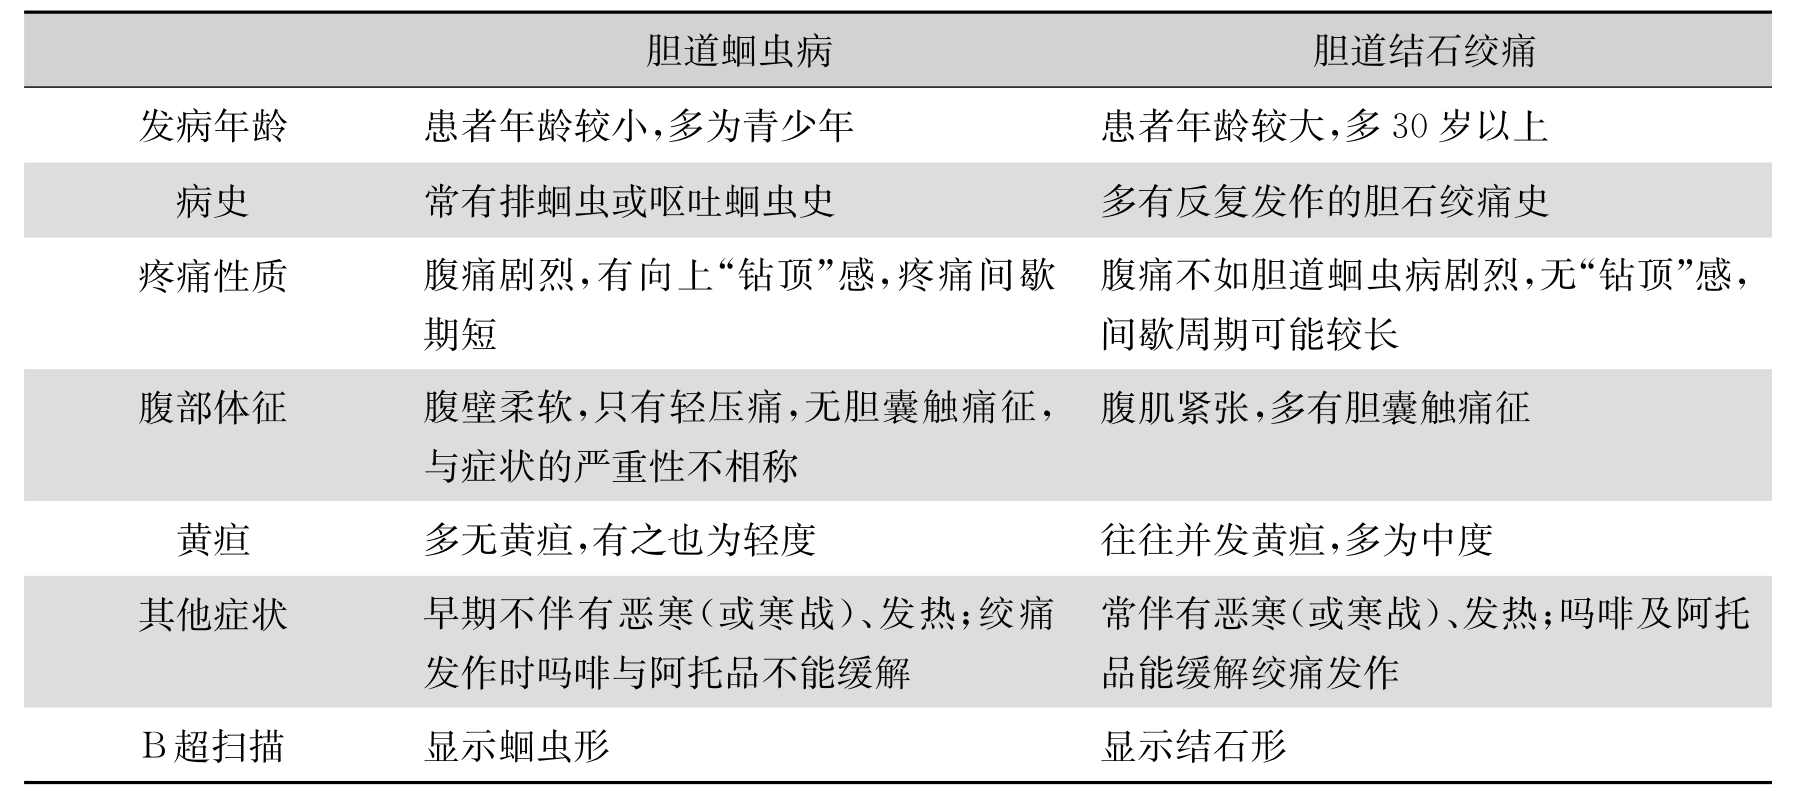
\includegraphics[width=5.97917in,height=2.66667in]{./images/Image00144.jpg}
\end{table}

\paragraph{五、胆石绞痛}

胆石症是胆道系统中最常见的疾病。我国胆石症男女性发病率大致相近,以20~40岁较多。胆石形成的原因尚未完全明了,蛔虫与华支睾吸虫对结石形成的作用已肯定,脂肪代谢障碍仍是重要的因素。

胆石症的临床表现决定于胆石的位置、大小、有无阻塞和炎症等。结石可位于胆囊、胆总管、肝管或肝内胆管。据国内统计,在胆囊炎病例中,70\%有结石存在。胆囊结石绞痛是阵发性上腹或右上腹绞痛,疼痛常向右肩部放射。多在夜间发作,其原因是平卧时,胆石由于重力关系滑进胆囊漏斗部造成阻塞。伴有恶心、呕吐,约50\%~60\%患者有发热,但往往在发病后一段时间才出现。

胆总管结石主要临床表现是上腹部或右上腹部阵发性剧烈绞痛伴阻塞性黄疸,寒战与发热。如疼痛、黄疸、寒战与发热都具备,称为夏科(Charcot)综合征。

胆石绞痛在临床上须与肠绞痛、肾结石绞痛、胰腺结石绞痛相鉴别(表\ref{tab25-5})。

B超检查可显示胆囊结石和胆管结石。X线检查对胆石症的诊断意义也大。含钙质的胆石在X线平片上呈不透X线的阴影;MRCP、ERCP或PTC胆道造影可发现透X线的胆管结石影像。

\paragraph{六、急性胆囊扭转}

胆囊扭转是一种罕见的急性胆道疾病,国内仅有少数病例报告。此病多发生于老年人,女性多见,且多为瘦长体型的人。胆囊完全性扭转的患者以右上腹剧痛而突然起病,腹痛呈持续性绞痛,多数放射至肩背部,伴有恶心、呕吐。体检右上腹腹肌紧张,有时在发病2小时内于胆囊区便可触到一压痛明显、梨形、可随呼吸移动的包块。患者过去无胆石症病史。疼痛发作开始时一般无发热与白细胞增多。此病术前诊断比较困难,尤其与胆石症并发急性胆囊炎不易鉴别,往往需在手术时方能确诊。

\begin{table}[htbp]
\centering
\caption{胆石症、肠梗阻、肾结石、胰腺结石绞痛的鉴别}
\label{tab25-5}
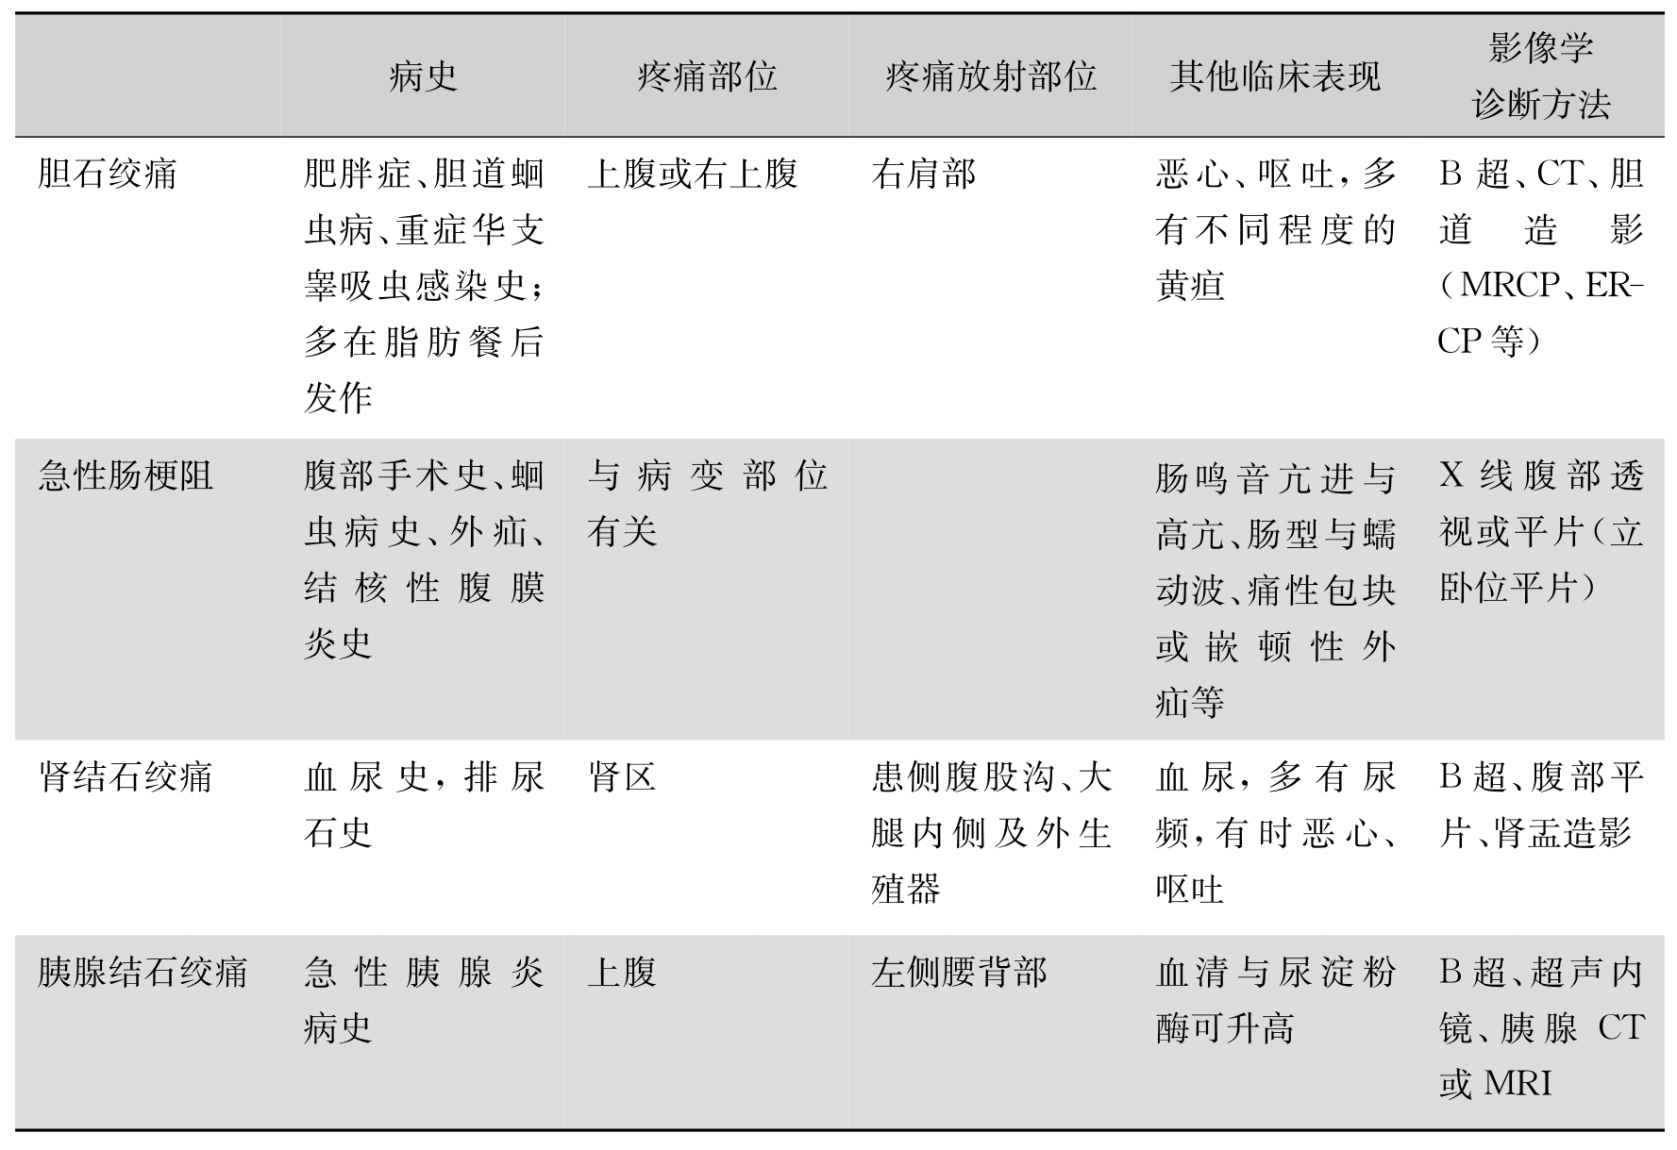
\includegraphics[width=5.91667in,height=4.05208in]{./images/Image00145.jpg}
\end{table}

\paragraph{七、肾与输尿管结石}

绞痛是肾与输尿管结石最主要的症状。绞痛一般发生于肾与输尿管结石的同侧腰部。较大的肾结石在肾盂内移动性较小时,疼痛多为钝痛,有时可无症状。较小的肾结石,在肾盂内移动性较大时,易引起肾盂输尿管连接部梗阻,与输尿管结石一样,可出现肾绞痛。肾绞痛是一种突然发生的剧烈疼痛,其特点是急性间歇性发作,疼痛从患侧腰部开始沿输尿管向下腹部、腹股沟、大腿内侧、睾丸或阴唇放射。持续几分钟,数十分钟,甚至数小时不等。发作时伴有恶心、呕吐、出冷汗、苍白、辗转不安,有时可出现休克。血尿是此病的第二个主要症状,输尿管结石比肾结石更易引起血尿,肉眼血尿也较多见。体检患侧肾区(脊肋点)或输尿管压痛点有压痛,但通常无肌紧张与白细胞增多。少数患者的发作类似肠梗阻,发作时肠鸣音亢进,但有血尿,与肠梗阻不同。如患者突然发生一侧腰部绞痛,并有上述的特殊性放射痛,肾区或输尿管有压痛,应首先考虑肾或输尿管结石。

过去尿中有排出结石或小砂粒病史,典型绞痛发作时又证明有血尿,则可确诊。如无上述的典型病象,B超和X线检查(X线腹部平片,静脉肾盂肾盏造影)是诊断此病的重要方法。

右侧肾与输尿管结石可与急性阑尾炎相混淆。阑尾炎的疼痛一般不如结石绞痛严重,无上述的特殊性放射痛,局部肌紧张与压痛明显,无血尿,可与此病相鉴别。

\paragraph{八、大网膜扭转}

大网膜扭转临床上少见。由于大网膜的右半部分长于左半部分,故扭转多发生于右半部分。大网膜扭转可分为原发性和继发性两类。原发性大网膜扭转:①形态异常如网膜上有一舌形突出,副网膜,双层网膜,带窄蒂的大而厚的网膜及肥胖者大网膜上有不规则的脂肪沉积等;②网膜上静脉曲张而动脉正常;③剧烈运动、突然改变体位、过饱后引起肠蠕动、咳嗽等使腹内压增高等因素,引起大网膜移动。原发性大网膜扭转均为单极的,只有1个固定点。继发性大网膜扭转,多由于大网膜与腹腔某一病灶如肿物、炎性病灶、疝囊、手术后切口或瘢痕之间产生粘连,这样形成了2个固定因素(即为双极的),在2个固定点之间的网膜发生扭转。各种内疝或外疝、肥胖、大网膜囊肿、大网膜变窄或形成带状是此病发生的主要因素;外伤及过度用力是发病的诱因。疼痛初始较轻,以后逐渐加剧,很少发生剧烈腹痛。疼痛部位多较固定,可于卧位或弯腰而缓解。发病可于体位突然转动或突然用力后即开始。疼痛可于发病后数小时甚至数天内消失或缓解,以后可再度出现。体检在右侧腹部有压痛及反跳痛,以右下腹部为明显。有时可扪及包块。体温、脉率及白细胞总数可稍升高(10
000~15 000/mm\textsuperscript{3}
)。如患者年龄在20~50岁之间,身体肥胖,发病较急且迅速局限在右下腹部,疼痛逐渐增加,病情发展缓慢,胃肠症状不显著,体检时可发现局部有一不明显的包块,较阑尾脓肿出现时间为早,应想到本病的可能。

本病最常误诊为急性阑尾炎。此外,尚须与急性胆囊炎、急性胰腺炎、胃十二指肠溃疡穿孔、梅克尔憩室炎、卵巢囊肿扭转等相鉴别。一般都经手术探查而确诊。

\paragraph{九、急性脾扭转}

急性脾扭转罕见,多发生于游动脾的基础上。患者出现暴发性急腹症症状,在女性常被误诊为卵巢囊肿扭转。由于腹肌紧张,以致未能触及脾脏的形状,是诊断困难的重要原因。

\paragraph{十、卵巢囊肿扭转}

卵巢囊肿扭转发生于体积较小、活动而蒂较长的囊肿。临床上如常自觉下腹部有肿块的女性患者,突然发生下腹剧烈持续性疼痛,不敢活动时,应注意卵巢囊肿扭转的可能性。此病疼痛一般位于下腹,非常剧烈,患者甚至可发生休克。如扭转严重,囊肿可发生坏死而出现腹膜炎征象。腹部检查患侧下腹部有压痛,可触及痛性肿块。阴道检查触及一圆形、光滑、活动而有明显触痛的肿块,有时甚至可扪到有触痛的扭转蒂部,对卵巢囊肿扭转有确定的诊断意义。

右侧卵巢囊肿扭转易误诊为急性阑尾炎。急性右下腹痛的女性患者,如临床表现不符合急性阑尾炎,应作妇科检查。

\paragraph{十一、妊娠子宫扭转}

妊娠子宫扭转临床上非常罕见,国内仅有少数病例报告。其临床特点是:①妊娠期间突然发生全腹持续性不可忍受的剧痛,伴有呕吐;②有面色苍白、冷汗、血压下降,甚至晕厥等急性内出血症状;③腹围大于妊娠月数,腹壁柔软无肌紧张,全腹有压痛,无宫缩;④阴道检查,宫颈位置很高,宫口紧闭,特别是内口,无分泌物。

\protect\hypertarget{text00197.html}{}{}

\subsection{78.4 腹腔脏器破裂出血}

局限性急性腹痛常伴轻中度腹膜刺激征(部分老年人或病情严重者,如合并休克,腹膜刺激征可不明显),伴苍白、冷汗、手足厥冷、脉搏细数、进行性红细胞与血红蛋白减少、休克,提示腹腔脏器内出血所致的急性腹痛。如有怀疑患者,可行腹腔穿刺,抽出不凝血性液体可确诊。有肿瘤病史(尤其是肝癌患者)应注意肿瘤破裂出血;有外伤史者多注意肝、脾破裂;有停经史(少数可无停经史)生育期已婚女性多注意异位妊娠破裂出血,生育期妇女还应注意黄体破裂出血可能。出血偶尔为自发性。

\subsubsection{一、肝破裂}

\paragraph{(一)肝癌破裂}

肝癌患者如突然出现剧烈腹痛,伴有血腹及腹膜刺激症状,则提示有肝癌破裂。此病的疼痛初为右上腹剧痛,以后扩展至全腹,呈持续性胀痛;常伴有周围循环不足或出血性休克症状,腹部体检发现腹部压痛、腹肌紧张较轻,肠鸣音有时反而加强,出血量多时有移动性浊音与进行性贫血。腹部X线透视膈下无游离气影,可与胃肠道穿孔相鉴别。B超、CT或MRI等影像学检查发现肝脏占位性病变和腹水,诊断性腹腔穿刺发现血腹有助于诊断。

\paragraph{(二)肝脏海绵状血管瘤破裂}

肝脏海绵状血管瘤少见。肝脏海绵状血管瘤破裂时也可引起急性右上腹疼痛,常伴有内出血休克症状与腹膜刺激征。

\subsubsection{二、脾破裂}

脾破裂发生于脾大基础之上,暴力作用是直接的原因,其来源不外乎人为的伤害,如殴斗、枪伤、刺伤等,以及意外的伤害,如车祸、跌伤、挤压、牛角刺伤等。脾破裂的主要临床表现是腹痛、急性贫血和休克(出血量常较大)。腹痛早期常限于左上腹,以后随出血量的增加而遍及全腹,疼痛可放射至左肩部。休克患者则腹痛程度较轻。腹部的主要体征是腹胀,呼吸运动减弱,全腹压痛与反跳痛,腹肌紧张(尤其左上腹最显著),移动性浊音,左上腹有固定性浊音。紧压颈部左侧胸锁乳突肌两下脚之间出现明显压痛,而紧压右侧相对应点无压痛,对脾破裂的诊断可有帮助。大量出血时周围血中红细胞与血红蛋白迅速下降。在临床上疑有脾破裂而未能确诊时,可用小型穿刺针于左下腹部有移动性浊音部作诊断性穿刺。如能吸出血液,可证明为腹腔内出血。综合病史与全面的临床检查,结合B超、CT或MRI等影像学检查阳性和诊断性腹腔穿刺发现血腹有助于诊断可作出脾破裂的诊断。有时须经手术探查才能确定为脾破裂,并与肝左叶或左肾破裂出血相鉴别。肾破裂主要表现为外伤后腰腹部剧痛,肾区压痛与肌紧张,血尿,有时休克,或逆行肾盂造影有助于诊断。如脾破裂为包膜下出血,则表现为进行性脾大、持续性左上腹疼痛与压痛、进行性贫血,而无上述的情况。

\subsubsection{三、异位妊娠破裂}

异位妊娠破裂是较常见的严重急腹症之一,不少患者首先到内科就诊,若不注意往往容易漏诊或误诊;异位妊娠破裂的盆腔内积血不引起强烈的腹膜刺激,是易于忽略的原因之一。国内报告一组1010例异位妊娠,约80\%发生于有分娩史或流产史的妇女,3/4有不孕症(以3年以上不孕者作为不孕症),发病年龄多在26~35岁,异位妊娠破裂约80\%在妊娠两个月内发生,但也有不到一个月的。异位妊娠破裂有三个主要症状:急性腹痛、阴道流血及停经。此组97\%有腹痛,大多位于全下腹,其次为右下腹、全腹部与左下腹等处。腹痛常自出血部位开始,向全腹扩展,呈持续性胀痛,严重者疼痛剧烈,乃至发生休克。约80\%患者有阴道不规则流血,大多数量少、暗褐色,呈点滴状,常持续很久。常伴有脉细数、出冷汗、晕厥等急性内出血症状。腹部检查下腹部有明显压痛,出血量多时有移动性浊音,腹肌紧张不一定存在。阴道检查发现宫颈有举痛,后穹隆饱满膨出,触痛显著,或子宫体旁触及一边缘不清的肿块。结合停经史和尿中绒毛膜促性腺激素(HCG)检测阳性,腹腔穿刺或后穹隆穿刺发现不凝固的血液即可确诊。

有些异位妊娠破裂出血,恰发生于正常月经周期内,最易误认为正常的月经来潮。因此,凡平时无痛经的妇女,尤其不孕症者,一旦月经来潮时发生显著的下腹痛、晕厥等症状,应注意异位妊娠破裂的可能,须进一步作有关的检查以明确诊断。疑为异位妊娠而患者尿中绒毛膜促性腺激素(HCG)增高,则应作超声检查。我院对22例临床疑为异位妊娠,全部作灰阶超声体层显像检查,均符合异位妊娠的诊断,随后经手术或临床追踪加以证实。

\subsubsection{四、卵巢破裂}

卵巢破裂在病理学上可分为滤泡破裂与黄体破裂。后者较前者为多见,且较多发生于右侧。卵巢破裂多发生于14~30岁之间的女性。文献报道滤泡破裂较多见于未婚者,而黄体破裂较多见于已婚者。卵巢破裂的主要症状是突然发生的剧烈下腹痛,伴有不同程度的恶心与呕吐。患者全身状态一般较好,但由于腹痛和内出血,往往表现不同程度的烦躁不安。体温及白细胞轻度增高。出血严重者可引起血压下降甚至休克,但少见。腹部检查患侧下腹部有压痛,如为右侧卵巢破裂,则压痛点常在阑尾压痛点下方约两横指处。腹肌紧张不显著;由于出血后血液在腹腔内引起非炎症性肠道刺激,使肠鸣音增强,但不高亢。如出血量较多,可出现移动性浊音。阴道检查发现宫颈坚实,无显著触痛,卵巢有时肿大并有触痛,附件无肿块。

右侧卵巢破裂常被误诊为急性阑尾炎。下列临床表现可与急性阑尾炎相鉴别:①卵巢破裂的腹痛多为突然发生,与阑尾炎的起病不同;②卵巢破裂腹痛开始即位于下腹部,而转移性腹痛支持急性阑尾炎腹痛,即先出现于上腹痛或脐周,以后才转移到右下腹;③卵巢破裂出血时,积血刺激子宫直肠凹陷,引起子宫、直肠、膀胱等收缩,故常有下腹部下坠感或里急后重;④卵巢破裂腹部压痛位置与范围比急性阑尾炎低而广泛,腹肌紧张不明显,恶心、呕吐也较轻,但出血、失水及休克症状则较阑尾炎为重。

卵巢破裂出血在临床上不易与异位妊娠破裂鉴别,下列几点可供参考:①发病与月经周期的关系甚有诊断价值,黄体破裂出血可发生于排卵后任何时期,大多发生于月经周期末一周内,而卵巢破裂常发生于排卵期,约在月经周期的第三周,特别在12~18天之间;②异位妊娠一般有停经史;③卵巢破裂多无阴道流血,而异位妊娠多有阴道流血;④上述症状与体征如发生于无性生活史的女性患者,则可排除异位妊娠破裂;⑤异位妊娠破裂常有尿HCG水平升高或检测阳性,B超有时可发现异位妊娠胚胎。少数疑难病例须经手术探查方能鉴别。

\protect\hypertarget{text00198.html}{}{}

\subsection{78.5 腹腔脏器血管病变(最常见为急性缺血性肠病)}

慢性心瓣膜病伴心房颤动、亚急性细菌性心内膜炎、高血压动脉硬化、肝硬化门脉高压或腹部手术后等情况下发生急性腹痛时,需考虑腹腔内脏器血管发生痉挛、梗死或血栓形成的可能性。如有血便,常由于肠系膜血管阻塞所致。

\subsubsection{一、肠系膜动脉急性阻塞}

肠系膜动脉急性阻塞临床上罕见,此病以急性腹痛为主要的临床表现。腹痛发生急骤,且呈持续性,通常有明显的阵发性加剧。疼痛位置视病变部位而异,一般为弥漫性,不似胆绞痛、肾绞痛与胃十二指肠溃疡疼痛具有显著的局限性,疼痛非常剧烈,使用大量的镇痛剂或解痉剂也不能缓解,常伴有恶心与呕吐。有的呕吐物与粪便为血性。体检常发现腹部膨隆性肌紧张及压痛,有时尚有肠鸣音减弱或消失,肠胀气,腹部可触及到面团样肿物。高热、白细胞增高及核左移也常出现。

肠系膜动脉急性阻塞大都由于栓塞引起,原发性血栓形成较少,病因多为心瓣膜病、心房颤动、亚急性细菌性心内膜炎、心肌梗死后心壁血栓形成等,少数由于动脉硬化所致。因此,器质性心脏病患者伴有心房颤动及各器官的多发梗死,如同时出现腹部持续性剧痛,应考虑肠系膜动脉血栓形成。

\subsubsection{二、肠系膜动脉粥样硬化}

肠系膜动脉粥样硬化可引起间歇性急性腹痛,临床上罕见。其发病机制与间歇性跛行相似。腹痛常发生于饱食之后,但也可无明显的诱因。患者同时有全身性动脉粥样硬化的表现。

\subsubsection{三、肠系膜静脉血栓形成}

肠系膜静脉血栓形成(MVT)发病多与门脉高压症、腹部手术或外伤后(尤以脾切除术后)、血液高凝状态等有关。其他少见原因为充血性心力衰竭、心肌梗死、红细胞增多症、糖尿病等。国内已有数组病例报告,最早、最突出的症状为腹痛,且持续时间长。腹痛可为局限性或全腹性,呈间歇性绞痛,但不剧烈。患者很少因突发性腹痛而就诊。大部分患者入院前已有较长时期的腹痛史,解痉剂疗效常不佳。约半数患者有恶心、呕吐。少数患者可有腹泻及便血。腹痛程度与腹部体征不相称是许多患者共有的表现。一般先作腹部平片检查以排除溃疡穿孔与结石梗阻。多普勒超声检查有一定参考价值。CT、MRI可显示门静脉系统的血栓,还可观察到肠系膜水肿,尤其是胃肠道CT、MRI对肠系膜静脉血栓形成和侧支静脉、异常肠段的判断正确率高达90\%以上。选择性肠系膜上动脉造影对诊断MVT价值有限,在动脉内注入血管扩张药物以减轻动脉的收缩,据此可区别动脉性缺血还是静脉血栓形成。

由于影像学及选择性血管造影技术的进展,使MVT在发生肠坏死之前作出诊断:近年来已有通过导管注入肝素、尿激酶、血管扩张药治疗MVT成功的报告。目前及时手术行肠段切除仍是治疗MVT最有效的方法。

\subsubsection{四、急性门静脉血栓形成}

急性门静脉血栓形成可发生于脾脏切除后(特别是原来血小板数正常的患者)、门腔静脉吻合术后、化脓性门静脉炎的病程中,或偶发于全身感染如伤寒、产褥热之后。起病急骤,其临床特点是剧烈腹痛、发热、腹胀、血性腹泻、轻度腹肌紧张,迅速发生而量多的腹水与脾大。腹痛一般多位于右上腹(参见第92节)。

近年来国内有文献报道10例患者,主要表现为急性中至重度中上腹部持续性疼痛,可伴有恶心、呕吐及上消化道出血。特征与腹痛程度不平行,仅表现为轻度腹部压痛,无反跳痛,肠鸣音无异常改变。

\subsubsection{五、急性肝静脉血栓形成}

肝静脉血栓形成十分少见,国内仅有少数病例报告。急性肝静脉血栓形成多骤然发病,其主要临床特征是:急性上腹部剧烈绞痛,呕吐,肝大与迅速发生、量多、不易消退的腹水(参见第92节)。

\subsubsection{六、脾梗死}

脾梗死的主要临床表现是突发性腹痛伴有急性脾大。疼痛位于左上腹,呈剧烈的刺痛,常向左肩胛部放射,深呼吸或转动体位可使疼痛加剧。脾区可听到摩擦音。如慢性心瓣膜病合并心房纤颤的患者,或亚急性细菌性心内膜炎的患者,突然发生左上腹疼痛,急性脾大,脾区有摩擦音,脾梗死的临床诊断便可成立。

\subsubsection{七、肾梗死}

临床上如慢性心瓣膜病合并心房纤颤的患者,或亚急性细菌性心内膜炎的患者,突然发生腰部疼痛,应注意肾梗死的可能性。疼痛位置多在腰部或胁腹部,性质类似肾绞相当剧烈。如同时发现有血尿及其他脏器的栓塞现象,则诊断大致可以确定。

\subsubsection{八、腹主动脉瘤}

腹主动脉瘤在中年人常为梅毒性,而老年人常为动脉硬化性;此病可引起剧烈的腹痛。疼痛多位于上中腹,具有钻痛性质,当渗血或破裂时疼痛极为剧烈,常位于脐周或背后相当于渗血或破裂部位的水平。触诊可在上、中腹部触及小儿拳头大的搏动性包块,按之可引起腹痛发作。在腹部包块上可听到滚筒样杂音,对诊断有重要价值。由于腹痛常突然发作,故须与胰腺结石相鉴别,但后者无搏动性肿块与杂音,X线摄片可发现胰腺结石阴影。腹主动脉瘤可应用多普勒超声、CT、MRI或腹主动脉造影以确定之。

\subsubsection{九、夹层主动脉瘤}

夹层主动脉瘤少见,临床诊断也较为困难。患者大多为40岁以上男性。一部分病例有腹部症状,可被误诊为急腹症。中年以上的高血压动脉硬化患者,发生急性剧烈腹痛,伴有休克征象而血压不下降者,应警惕夹层主动脉瘤的可能。如患者有类似肠梗阻的表现,而疼痛向上、下肢放射,一侧桡动脉脉搏消失,心电图及血清心肌酶学检查无急性心肌梗死征象,则诊断大致可以确定。腹部检查腹肌可轻度紧张,但不如急性腹膜炎明显。多普勒超声对本病有一定的诊断价值,而CT、MRI对确诊更有帮助,准确率超过90\%,有时几乎达到100\%。

\protect\hypertarget{text00199.html}{}{}

\subsection{78.6 腹腔脏器其他疾病}

\subsubsection{一、急性胃扩张}

急性胃扩张通常发生于暴食之后。有时进食并不太多,而在进食前后由于情绪波动、剧烈疼痛、受寒、腹部外伤等不良刺激也可引起此病。临床特点是:患者在暴食后1~2小时左右,突然发生上腹部或脐周持续性胀痛或隐痛,可阵发性加剧,伴饱胀感,呕吐、呃逆。呕吐的特点是频繁而呕吐量不多,腹胀不减轻。烦渴欲饮,但随饮随吐。体检可见腹部膨胀,尤以上腹部为显著,全腹仅有轻度压痛,叩诊呈鼓音并有振水音。起病时腹部膨胀,但腹肌柔软,与胃、十二指肠溃疡穿孔不同;无肠型和肠鸣音亢进,可与急性肠梗阻相区别;无腹泻,而腹胀显著,可与急性胃肠炎鉴别。X线检查可见扩大的胃泡和胃内大量食物残渣影像,对诊断有帮助。如有腹膜炎征象或胃肠减压无效,应考虑手术治疗。

\subsubsection{二、痛 经}

痛经大多数在经前一、二天,或月经来潮的第一天开始,于经期中逐渐减轻以至消失。也有在经后期或经期后出现的。历经数小时至一天不等。痛经部位多在下腹部,有时放射到腰骶部、上腹部、外阴、肛门及其他部位,严重时可伴有呕吐及膀胱直肠激惹症状。极少数患者可有面色苍白、出冷汗,甚至晕厥。腹部检查无腹肌紧张,直肠指检盆腔无炎症性征象。患者过去月经期间有同样的疼痛发作史,对诊断有重要帮助。

\protect\hypertarget{text00200.html}{}{}

\section{79 腹外脏器疾病(包括全身性疾病)}

腹外脏器疾病(包括全身性疾病)所致的急性腹痛,以胸部疾病所致的反射性腹痛与中毒与代谢疾病所致的痉挛性腹痛为多见,常伴有腹外其他器官病征,而无明显的腹部压痛、反跳痛、腹肌板样硬、肠鸣音减弱或消失等急性腹膜炎征象。

\subsection{79.1 胸部疾病}

\subsubsection{一、肋间神经痛}

肋间神经痛可在该神经分布的区域内出现剧烈疼痛,并伴有肌痉挛与压痛。如病变发生于支配腹壁的肋间神经,临床表现易与腹部脏器炎症所致的急性腹痛相混淆。但患者一般无发热、呕吐,白细胞不增多,压痛与肌痉挛不局限于腹部,而遍及该神经的支配区,神经接近体表处有压痛,并有皮肤感觉过敏现象。如出现带状疱疹(应注意隐匿性带状疱疹),可出现相应区域腹痛。图\ref{fig25-5}鉴别胸部疾病与腹部疾病所致右侧腹痛的检查法(腹部疾病时,从左向右压引起腹痛)更明显。

\begin{figure}[!htbp]
 \centering
 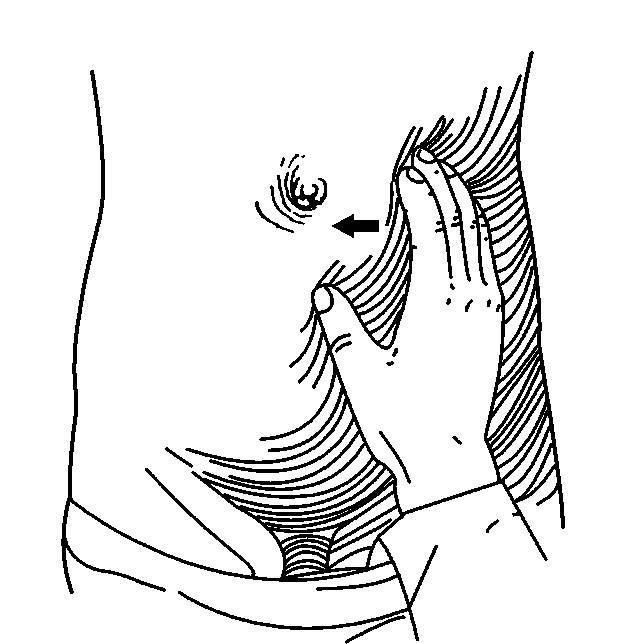
\includegraphics[width=2.08333in,height=2.13542in]{./images/Image00146.jpg}
 \captionsetup{justification=centering}
 \caption{鉴别胸部疾病与腹部疾病所致右侧腹痛的检查法\\{\small (腹部疾病时,从左向右压引起腹痛)}}
 \label{fig25-5}
  \end{figure} 



\subsubsection{二、膈胸膜炎}

膈胸膜炎是一种特别类型的胸膜炎,较多并发于大叶性肺炎。病变都在肺下叶,腹痛多见于发病的早期。此病的特点是:①患侧上腹部持续性疼痛;②疼痛往往向患侧肩部放射,患侧肩部有压痛点;③患侧膈运动受限,膈现象消失。右膈胸膜炎时,检查者用手压患者左下腹部,并从左向右压诊(图\ref{fig25-5}),如为胸部疾病所致的右侧腹痛,则不引起疼痛,而腹部疾病所致者则引起疼痛。有膈胸膜炎有时可与胃、十二指肠溃疡或阑尾炎急性穿孔混淆;特别是伴有黄疸时,易误诊为急性胆囊炎。患者腹痛前常先有发热、咳嗽,伴有肺部体征,腹部深触诊并不比浅触诊更痛,在发病后24~36小时X线检查可发现肺部阴影,可明确与以上的急性腹痛相区别。

\subsubsection{三、急性心肌梗死}

少数急性心肌梗死患者可仅表现为上腹部的急性疼痛,伴有恶心、呕吐,甚至可有腹肌紧张,上腹压痛,类似外科急腹症。这种情况可被误诊为胃、十二指肠溃疡穿孔、急性胆囊炎与胆石症、急性胰腺炎、急性肠梗阻。因此,临床上遇见40岁以上的患者,罹患病因未明的急性腹痛,尤其是有高血压、动脉粥样硬化或过去有心绞痛发作史者,要警惕急性心肌梗死的可能性。体检常可发现心音减弱,左心增大,部分患者可出现奔马律、心律失常,均有重要的鉴别意义。高血压不一定存在。部分患者可发生急性左心衰竭,或血压下降,甚至休克。心电图的特征性表现或(及)血清心肌酶活性增高,对此病有重要诊断价值。

\subsubsection{四、急性心包炎}

急性心包炎可出现上腹部疼痛,特别是急性非特异性心包炎(参见第55.4节),且可以急性腹痛为主要表现,伴有腹肌紧张、压痛、出汗、面色苍白等症状。腹痛为持续性或阵发性,多位于上中腹部,有时位于右下腹或全腹。心包炎引起腹痛的原因是炎症侵及膈胸膜,以及心包积液压迫下腔静脉与部分肝静脉,导致肝淤血、牵张肝包膜所致。

国内报道一组106例急性心包炎中,5.7\%以急性腹痛为特征,此时易与急性胆囊炎、急性胰腺炎、胃十二指肠溃疡穿孔、急性阑尾炎等相混淆。

如体检发现心包摩擦音,符合纤维素性心包炎的诊断。如患者有颈静脉怒张、心界扩大且随体位而改变、心音遥远、肝大、下肢水肿、奇脉与脉压小等病征,则符合渗出性心包炎的诊断。X线检查与心脏超声波、CT和MRI等检查对诊断渗出性心包炎也有帮助。诊断性心包穿刺抽得心包积液则诊断明确。

\subsubsection{五、急性右心衰竭}

各种原因引起的急性右心衰竭导致急性肝淤血时,迅速肿大的肝脏可出现显著的和发展较快的右上腹疼痛,并可放射至右背部。

\subsection{79.2 中毒及代谢障碍疾病}

\subsubsection{一、慢性铅中毒}

铅绞痛是慢性铅中毒最常见的症状,发生率比瘫痪多10倍。铅绞痛发作常在便秘后数天突然出现。疼痛多位于脐周或脐下方,呈阵发性,每隔几分钟以至数小时发作一次,可断续存在几天至数周。腹痛可甚剧烈,用手紧压腹痛处,痛可减轻,常伴有呕吐、出汗。体检可见牙龈有铅线,皮肤黏膜苍白超过贫血的程度(所谓铅苍白)。腹部平坦、柔软或稍紧张,无固定压痛点。铅绞痛的诊断主要根据长期或过量铅接触史,上述的临床表现以及24小时尿铅排量≥0.39μmol/L。铅绞痛的漏诊多由于对病史的忽略,例如漏诊进食含铅的中药(如黄丹、樟丹、密陀僧)及漏诊摄入含铅汽油所致的铅绞痛亦曾有之。

\subsubsection{二、铊(thallium)中毒}

急性铊中毒的症状与铅中毒的症状相似,如同时有顽固性便秘,可与血卟啉病相混淆。铊的盐类多用为毒鼠药及脱毛剂,误食可引起中毒,国内也有报告。内服大量铊盐的急性中毒患儿常在数小时到24小时内出现症状,如恶心、呕吐、口炎、腹痛、腹泻,可有出血性胃肠炎(或有便秘),皮肤、黏膜出血,心动过速及其他心律失常,血压升高,肝、肾损害,脱发,多发性神经炎症状。部分患儿发生急性铊脑炎,出现头痛、嗜睡、精神错乱、幻觉、惊厥、震颤、谵妄、昏迷等。重症患儿并有肺水肿、呼吸困难以至呼吸衰竭、休克等,可于数日内死亡。若因长期应用铊盐治疗发癣而中毒,其症状发作缓慢,患儿可有疲乏,抑郁,失眠,激动,恶心、呕吐,感觉异常,肢端疼痛,手指震颤,肌肉无力,眼睑下垂、斜视,瞳孔散大,面肌强直,球后视神经炎,视神经萎缩、失明。此外,可有贫血,牙龈炎及牙龈蓝线,脱发,指、趾甲显现苍白痕或脱落,各种皮疹及表皮角化,皮肤有瘀斑或瘀点,肝、肾损害,糖尿等。此外,可有痴呆、甲状腺功能不全、发育迟钝及睾丸萎缩等。轻症可完全恢复,发生球后视神经炎后,视力大都减退。急性中毒患儿约有半数出现不同程度的各种后遗症。根据确切的铊接触史、典型的临床表现、参考尿铊或其他生物材料中铊的测定,并排除其他病因所致周围神经病,铊中毒的诊断一般不困难。

铊中毒的严重程度,目前参考职业性急性铊中毒的分级标准,具体如下:

轻度中毒:除具有头晕、头痛、乏力、食欲减退、下肢沉重症状外,同时具备以下任何一项者:①四肢远端特别是下肢麻木,痛觉过敏,痛觉、触觉减退呈手套、袜套分布或跟腱反射减弱;②神经-肌电图显示有神经源性损害。

重度中毒:上述症状加重,具备下列一项表现者:①中毒性脑病或中毒性精神病;②四肢远端明显肌肉萎缩并影响运动功能,或多发性脑神经损害;③肌电图显示神经源性损害并有较多自发性失神经电位;④伴有明显心、肝或肾损害。

鉴别诊断需要排除癔症、吉兰-巴雷综合征、血卟啉病、肉毒毒素中毒、糖尿病及铅、砷、二硫化碳、一氧化碳等中毒性疾病。

\subsubsection{三、糖尿病酮症酸中毒或乳酸性酸中毒}

糖尿病酮症酸中毒或乳酸性酸中毒引起腹痛多见于青少年患者,腹痛的特点是呈阵发性,相当剧烈,伴腹胀、恶心、呕吐等。产生腹痛的原因主要是酸中毒时伴有失钠、失氯、失水严重等水、电解质紊乱,导致肌肉痉挛所致。有时可伴有发热,白细胞增高,腹部压痛与腹肌紧张,甚至X线透视有肠液平面,可误诊为肠梗阻、急性腹膜炎、阑尾炎、胆囊炎、急性胰腺炎等急腹症;另一方面,糖尿病酮症酸中毒或乳酸性酸中毒患者也可并发外科急腹症。

下列几项特点有助于糖尿病酮症酸中毒或乳酸性酸中毒与外科急腹症的鉴别诊断:①糖尿病酮症酸中毒或乳酸性酸中毒发生前常有多饮、多尿的一段过程,而外科急腹症多突然发生;②糖尿病酮症酸中毒或乳酸性酸中毒,先呕吐后腹痛;而后者则多先腹痛后呕吐,或两者同时发生;③糖尿病酮症酸中毒或乳酸性酸中毒,pH值下降、碱失衡、尿糖强阳性、血糖明显升高、尿酮体阳性;而后者无此现象;④糖尿病酮症酸中毒或乳酸性酸中毒早期,症状经积极治疗3~6小时后便完全消失;如由外科急腹症所致,则症状仍继续存在;⑤糖尿病酮症酸中毒或乳酸性酸中毒常有糖尿病控制不佳(口干、多饮、多尿,伴有头晕、乏力等不适)或服用某些药物(如乳酸性酸中毒常与双胍类降糖药服用有关)。

有文献报道,11例糖尿病酮症酸中毒患者,年龄16~72岁,11例均以急性腹痛为首发症状,其中全腹痛2例,脐周痛3例,上腹痛5例,下腹痛1例;伴恶心、呕吐或腹泻9例,腹部压痛4例,轻度脱水7例,中度脱水3例,重度脱水1例。误诊疾病:急性胃肠炎、急性胰腺炎、急性阑尾炎、泌尿系结石、急性胆囊炎及急性原发性腹膜炎,误诊时间0.5~3天。

\subsubsection{四、尿毒症}

尿毒症也可引起反射性肠绞痛,但腹部压痛与腹肌紧张甚轻或无,并有尿毒症其他征象,诊断一般不困难。

\subsubsection{五、血卟啉病}

血卟啉病是临床少见的、原因尚未完全明了的代谢障碍疾病,一般认为与遗传有关。文献报道患者多为20~40岁的女性。国内报告大多数是急性间歇性肝性血卟啉病。血卟啉病主要临床表现有皮肤、腹部及神经系统等三大症候群。

皮肤症状主要由于感光过敏,表现为皮肤暴露部分的感光性皮炎(如红斑、疱疹、皮肤糜烂与色素沉着等)。皮肤损害多在婴幼儿时期出现。腹部症状群的特征是急性腹痛,可因服用巴比妥类药、酒精等诱发,常伴有恶心、呕吐与便秘。腹痛往往突然发生,可非常剧烈,常为绞痛性,也可呈紧缩性或重压样疼痛。腹痛的部位不固定,可在上腹部、脐周、左腹或右腹;有时疼痛在背部或膀胱,放射至外生殖器。有时仅有腹部重压感。腹痛持续时间由几小时至数天甚至数周不等。腹痛发作可仅一次或多次反复,间隔期可长可短。腹痛发作时小便呈红色,或小便暴露于阳光下变为红色。急性血卟啉病易误诊为外科急腹症,但此病腹痛无固定部位,无肌强直与反跳痛,腹式呼吸存在,也无白细胞增加与核左移现象。患者可有癔症样动作、肢体疼痛或麻痹、软弱、怕光、反射消失、神经衰弱或延髓麻痹症状。因此临床上遇到原因未明的急性腹痛患者,腹部检查腹壁柔软,无固定压痛时,应考虑此病的可能。

急性血卟啉病的确诊,有赖于发作期尿中卟胆原与尿卟啉检查。如两者均为阳性,则诊断明确。如尿中卟胆原阳性而尿卟啉阴性,也可诊断为本病。尿卟啉的检测须用分光镜。在技术条件受限时,尿卟胆原试验是简单而有诊断价值的试验。

近年来有报道,15例患者中,发病年龄15~67岁,病程80天~10年不等,绝大部分病例发病有明显诱因,主要为感染、药物、饥饿、精神刺激、妊娠、月经失调及饮酒等。临床表现主要是腹痛15例,伴腰背痛5例,腹痛常为绞痛、胀痛或刀割样疼痛,阵发性加剧,反复发作,部位不固定,多为脐周,亦可全腹,持续时间数小时至数日,少数达数周,间歇期几十分钟至数月不等。本组有神经精神异常4例,表现多样,呈忧郁、情绪不稳、烦躁不安,失眠、嗜睡、幻觉、谵妄和意识障碍等。尿卟啉定性试验(部分患者多次检测)15例全部阳性。

\paragraph{附:尿卟胆原试验}

在试管中加入患者尿液及尿胆原定性试剂(Ehrlich醛试剂)各3ml。在此混合液中再加入醋酸钠饱和水溶液6ml与氯仿5ml,混合之。如患者尿卟胆原阳性,则卟胆原醛存留于水层中呈红色。

\subsubsection{六、低血糖}

血糖过低有时也可引起剧烈腹痛,这种腹痛为一过性。患者无腹膜刺激征象,而伴有其他低血糖症状,补给糖类如葡萄糖后腹痛迅速缓解(参见第41章)。

\subsubsection{七、原发性高脂血症}

本病可发生剧烈的腹痛,类似急性阑尾炎或急性胰腺炎。其临床特征是:黄色瘤、脂血症性视网膜炎与肝脾大。有人认为患者血中类脂的物理改变,可使其颗粒结合起来引起血管梗死而致腹痛,亦有人认为剧烈的腹痛可能由于并发急性胰腺炎所致。

\subsubsection{八、低钙血症与低钠血症}

低钙血症或低钠血症有时也可出现急性腹痛。低钙血症可见于哺乳期妇女,腹痛发作时Chvostek征阳性,注射葡萄糖酸钙后症状迅速缓解,血钙测定多低于正常。低钠血症多见于热痉挛或其他失钠情况(如糖尿病、严重腹泻或呕吐等),注射生理盐水后腹痛即可缓解。

\subsubsection{九、麻醉品肠道综合征}

长期吸毒可引起胃肠道平滑肌痉挛而致急性腹痛,随后又可致胃肠长时期松弛、膨胀,并可引起肠绞痛或假性肠梗阻,这种临床情况也有称为麻醉品肠道综合征。曾有一组3例报告吸毒(海洛因、大麻)所致急性腹痛,1例误诊为急性阑尾炎而进行手术,2例被误诊为溃疡病穿孔,由于认识提高,经对症治疗后病情缓解。

\subsubsection{十、回盲肠综合征}

回盲肠综合征(ICS)又称中性粒细胞减少性回肠结肠炎,是发生在白血病治疗过程中的严重并发症,中性粒细胞减少时出现的以发热、腹泻、腹痛及转移性右下腹痛为主要症状的临床综合征。ICS的前驱症状不明显、少数患者反应迟钝。但病情进展快并很快出现败血症和中毒性休克。其发病机制未明确,有报道认为该病的发生与长期化疗、应用抗生素、中性粒细胞缺乏、血小板减少及凝血机制障碍等多方面因素有关,而回盲部组织疏松。血管稀少而淋巴组织丰富以及食物局部停留摩擦,故好发于此处。近来有文献报道,16例ICS患者,年龄13~54岁,合并急性细胞白血病12例,急性淋巴细胞白血病4例,全部患者均以转移性右下疼痛伴发热为首发症状,其中13例出现腹泻;9例在发病12h内出现中毒性休克症状,5例伴DIC。全部患者均有下腹压痛、反跳痛,其中5例于右下腹可触及包块。7例腹部超声于右下腹探及包块及液性暗区,X线检查可见肠袢气影,回盲部形态不规则;2例有不全肠梗阻表现;血培养10例无菌生长,2例为黏质沙雷菌,3例为表皮葡萄球菌,1例为白念珠菌。

\subsection{79.3 变态反应及结缔组织病}

\subsubsection{一、腹型过敏性紫癜}

本病患者绝大多数是儿童与青少年,男性多于女性。本病多发生于上呼吸道或胃肠道感染或进食某些食物之后。绝大部分患者都有皮肤症状,腹部症状也多见,且后者可作为首发症状而出现。疼痛常为发作性绞痛或钝痛,可甚剧烈,部位常不固定,多在左、右下腹或脐周,有时遍及全腹,一次发作多持续1~2小时,少有超过一天的。常伴有恶心、呕吐、腹泻,有时有便血或血尿。此病可误诊为急性阑尾炎、肠梗阻、内脏穿孔、腹膜炎、急性局限性肠炎等。腹型过敏性紫
癜的下列临床特点有助于与上述的急性腹痛相鉴别:①腹痛部位常不固定;②每次发作时腹部症状与体征的表现并不一致;③体征(腹肌紧张及强直)不如症状(腹痛、腹泻等)明显;④多数病例伴有相当明显的腹泻,与一般急腹症不同。此外约半数病例血中嗜酸性粒细胞增多,提示为过敏性疾病。如出现紫癜与关节肿痛,则鉴别更为容易(参见第115.2.2节)。

\subsubsection{二、腹型风湿热}

腹型风湿热临床上少见,患者以儿童为多,腹痛为主要的主诉。国内曾报告一组风湿热病例6\%出现剧烈腹痛。腹痛程度轻重不一,常伴有恶心、呕吐,有时腹泻。腹型风湿热的诊断有时甚为困难,尤其当腹痛发生于多发性关节炎、心肌炎、皮下结节、环形红斑等风湿热病征出现之前。凡年轻患者,尤其曾有风湿热病史者,如伴有高热、腹痛、白细胞增加与血沉率显著加快,应考虑腹型风湿热的可能性。此病虽有高热,而无腹肌紧张,压痛部位常不固定,血内嗜酸性粒细胞多无明显减少,可与严重的外科急腹症相区别。如患者同时出现部分或全部上述的风湿热病征,则可能性更大。心电图异常改变(如P-R间期延长、二联律等)以及血沉率与血清抗链球菌溶血素“O”滴度增高有助于诊断。如有上述临床表现的患者,经抗风湿药物治疗后,腹痛与发热随之缓解,则可诊断为腹型风湿热。

\subsubsection{三、结缔组织病}

结节性多动脉炎可引起不同程度的腹痛发作,发作不定时,也无定位。系统性红斑狼疮约半数病例有不同程度的腹痛,大多局限于脐周。偶尔疼痛相当剧烈,类似外科急腹症,可能并发无菌性腹膜炎症。

\subsection{79.4 急性溶血}

急性溶血由某些药物、感染或食物(如蚕豆)引起者较多,偶尔可由于输血错误所致。患者有恶寒或寒战、发热、恶心、呕吐,可伴有急性腹痛,并出现黄疸,白细胞增多,与急性胆囊炎相似,但患者无胆囊触痛征而有血红蛋白尿与溶血性贫血,黄疸也为溶血性,可以互相区别。

\subsection{79.5 神经源性与功能性胃肠病}

\subsubsection{一、腹型癫痫}

腹型癫痫第一次发作的年龄一般为7~8岁。此病临床上较少见,国内一组有20多例报告。腹型癫痫的临床特点是:①腹痛呈周期性反复发作,持续几分钟至几小时,发作与终止均较突然,疼痛多在脐周,也可涉及上腹部,常伴有恶心、呕吐、腹泻,间歇期腹部无任何症状与体征;②发作过程中或中止后,常可出现意识障碍、嗜睡、腹部或肢体肌肉跳动或抽动、偏头痛、流涎和吞咽咀嚼动作等表现;③实验室和各种辅助检查(包括超声、X线、CT、MRI、胃肠镜等多种检查)无器质性腹部病征发现;④在发作期作脑电图检查,可发现符合癫痫的脑电波,但须注意,脑电图正常不能完全排除此病;⑤抗癫痫特效药物有显著的疗效。在诊断方面,病史非常重要(包括家族史、产伤、脑部外伤、以往感染史等)。患者虽有剧烈腹痛,但却无发热、白细胞增多与胃肠梗阻征象,在腹痛间歇期宛如正常儿童。如多次大便检查未发现寄生虫卵,胃肠钡餐未见异常,而患者有上述病史,有必要作脑电图检查。

\subsubsection{二、脊髓疾病}

脊髓痨常见于结核或晚期神经梅毒,后者约在感染后5~15年发病。疼痛是此病早期特有的症状,但不限于腹部。疼痛呈闪电样,可非常剧烈,持续数秒至数小时,有时甚至数天之久。发生胃危象时,除有严重胃痛外,伴有剧烈的恶心与呕吐。有时患者觉胸部与腹部有束带感。危象通常无明显诱因而突然发生,又突然停止。发生肠危象时则表现为肠绞痛与腹泻。如不注意,可将脊髓痨胃、肠危象误诊为其他急性腹痛。阿-罗瞳孔、膝腱反射消失、脑脊液胶状金试验与血清梅毒反应阳性,可协助诊断。

有文献报道12例脊椎损伤中,均为女性,年龄75~88岁。全部病例均为主诉急腹痛,主要为突发的上腹部或脐部以上部位或单季肋区/双季肋区的疼痛,定位范围模糊不清,自发病开始至就诊时疼痛程度变化不大,一般尚可忍受,基本不影响进食和排便,部分患者伴咳嗽或变动体位时疼痛加剧,特别由卧位、坐位起立时,上腹疼痛更趋明显,但不伴有发热、头痛、头晕、心悸、胸痛、恶心、呕吐、腹泻与尿黄等症状。体检腹部软,肝脾均未触及,Murphy征阴性,但多伴有腹壁皮肤痛觉过敏,触摸皮肤即感觉疼痛,轻压脊柱疼痛不明显,较重压时有不同部位的轻度疼痛,四肢活动自如,多有诱因(如:提重物或滑倒后臀部着地史)。

\subsubsection{三、功能性胃肠病(参见第26章)}

功能性胃肠病常见于慢性腹痛,急性腹痛较少见,精神因素是重要的发病基础,须经较长时期的观察,慎重排除一切腹部器质性病变后方能确定诊断。

\protect\hypertarget{text00201.html}{}{}

\section{参考文献}

1.许乐,罗庆锋.老年人急性胰腺炎122例临床分析.中华老年医学杂志,2006,2:36-38

2.王林华.阑尾血吸虫病并发急性阑尾炎临床分析.中国血吸虫病防治杂志,2009,2:144,149

3.缺血性肠病中国专家建议(2011)协作组.老年人缺血性肠病诊治中国专家建议(2011).中华老年杂志,2011,11(1):1-3

4.李则夫.中药黄丹、樟丹、铅粉中毒11例报告.中华内科杂志,1982,21:366

5.马云龙.B超检查对阑尾炎诊治的指导意义.中华外科杂志,1993,31(9):589

6.王秀玲,等.慢性肠假性梗阻8例报告.中华消化杂志,1992,12(3):148

7.伍冀湘,等.肠系膜静脉血栓形成7例临床分析.中华外科杂志,1997,35(6):351

8.宋少柏.肠系膜上静脉梗死.中华内科杂志,1993,32(1):59

9.王荫槐,等.肠系膜静脉血栓形成的早期诊治(附16例临床分析).中华外科杂志,1997,35(7):443

10.宋少柏.肠系膜上静脉梗死.中华内科杂志,1993,32(1):59

11.高广文.急性肠系膜静脉血栓形成肠坏死11例诊治体会.中华消化杂志,1998,18(4):255

12.李茂亭,等.主动脉夹层动脉瘤临床研究.中华内科杂志,1994,33(6):385

13.陆雪林,等.系统性红斑狼疮腹部危象------附4例报告.中华消化杂志,1989,9(1):61

14.周晓东,等.急性间歇性卟啉症的诊断与治疗(附10例报告).中华消化杂志,1998,10(6):378

15.王农荣,等.急性腹痛为主要症状的血卟啉病15例报告.中华急诊医学杂志,2003,12(2):132

16.殷国田.以腹痛为主要表现的糖尿病酮症酸中毒11例误诊分析.临床荟萃,2003,18(10):590

17.李清云,等.结缔组织病所致急腹痛.中华消化杂志,1993,13(3):172

18.臧仁迅,等.中药引起铅中毒24例临床分析.中华内科杂志,1996,35(9):608

19.陈积圣,等.吸毒与急腹症附3例并文献复习.中华内科杂志,1995,34(1):46

20.张安忠,等.梗死性缺血性肠病26例临床分析.中华消化杂志,2005,25(3):171

21.李景南,等.肠系膜静脉血栓形成所致的腹痛的临床分析.胃肠病学,2003,8(2):90

22.马丽辉,等.白血病合并回盲肠综合征临床分析.中华内科杂志,2001,40(10):720

23.徐玲珍,等.脊椎骨折所致急腹痛的临床分析.中华消化杂志,2005,25(1):41

\protect\hypertarget{text00202.html}{}{}

